% Created 2017-08-23 Wed 23:57
% Intended LaTeX compiler: pdflatex
\documentclass[12pt]{report}
\usepackage[utf8]{inputenc}
\usepackage[T1]{fontenc}
\usepackage{graphicx}
\usepackage{grffile}
\usepackage{longtable}
\usepackage{wrapfig}
\usepackage{rotating}
\usepackage[normalem]{ulem}
\usepackage{amsmath}
\usepackage{textcomp}
\usepackage{amssymb}
\usepackage{capt-of}
\usepackage{hyperref}
\usepackage{graphicx}
\usepackage[utf8]{inputenc}
\usepackage[english]{babel}
\usepackage[a4paper, total={150mm,237mm}, left=30mm, top=30mm,]{geometry}
\usepackage{pdfpages}
\usepackage{color}
\usepackage[cache=false]{minted}
\usepackage{caption}
\usepackage{subcaption}
\linespread{1.3}
\widowpenalty10000
\clubpenalty10000
\setcounter{secnumdepth}{4}
\date{\today}
\title{}
\hypersetup{
 pdfauthor={},
 pdftitle={},
 pdfkeywords={},
 pdfsubject={},
 pdfcreator={Emacs 25.0.94.2 (Org mode 9.0.9)}, 
 pdflang={English}}
\begin{document}

\frontmatter

\includepdf[pages=\{1-\},scale=1.0]\{title-page.pdf\}

\part{Acknowledgments}
\label{sec:org84e8c84}

\begin{large}
Thanks to my family and friends for all the support throughout the past year, in
particular this last stretch.

Thanks to the MMT staff and lecturers for their tireless dedication. In
particular, thanks to Liam for guiding me through the sometimes stormy waters of
completing this thesis project.

Finally thanks to all my classmates for making this a memorable and enjoyable
year!
\end{large}


\tableofcontents
\cleardoublepage

\listoffigures
\cleardoublepage

\mainmatter
\part{Introduction}
\label{sec:orgf98f3fc}
\chapter{Introduction}
\label{sec:org4165008}
The traditional route for both recorded and performed musical expression has
been through playing a musical instrument. Through this simple but powerful
interface, ideas can be explored by the skilled practitioner in a free flowing,
intuitive manner. The ubiquity of high powered computers has led to a
fundamental change to this process, however. Electronic music can now be
produced entirely on a computer, enabling those without the background or
training to produce music to a professional standard. The affordances of
infinite editability and tweak-ability allows the novice producer to organically
build compositions through a process of trial and error. The requirement to
perform to a high standard is no longer necessary.

The primary tool of this new breed of electronic musician, is the Digital Audio
Workstation (DAW), a powerful software application for composing, arranging and
editing musical events and audio material, mixing tracks and applying audio
effects. To control this power, the electronic musician must master the vast
array of knobs, sliders, buttons and complex hierarchies of settings. This
complexity poses some difficult Human Computer Interaction (HCI) challenges both
for software developers and end users \cite{duignan_abstraction_2010}.

A common solution to this is to provide the user with real world metaphors in
the presentation of the interface. In this way, the highly abstract process that
takes place in digital systems can be grounded in a metaphorical language
understandable to the user. An extremely dominant metaphor is that of the analog
mixer and the hardware multi-track tape machine which have, since the mid-1990s,
become a mainstay construct in the interfaces of commercial DAWs
\cite{bell_journal_2015}. The effectiveness of this metaphor is evident in the
vast amount of music produced in this environment. There are some situations,
however, where the metaphor can get in the way and lead to another new, separate
layer of complexity that must, in turn, be managed by its users.

\chapter{Motivation}
\label{sec:orgf314316}
This leads to the central motivation behind the work on SonicSketch: that of
exploring alternative metaphors that support the early stage of music production
and fulfills the role traditionally filled by an instrument. In exploring these
alternative metaphors, an attempt is made to regain some of what is lost when
working directly with the computer without compromising the distinct advantages
it brings.

The intention is not to suggest that analog studio metaphors can be replaced, or
even that there is any reason that they should be. Instead, the intention is to
augment these rich metaphors with other metaphors more suited to certain stages
of the creative process. The need for such efforts is in some ways acknowledged
by mainstream DAW manufacturers. For instance Ableton Live, a highly popular DAW
application, has recently opened its application programming interface (API) to
allow other programs to create compatible files \cite{ableton_live_2017}. This
enables producers to work in diverse, idiosyncratic and perhaps less featured
environments more suited to the capturing of ideas and creative flow. The option
is open to then move freely to the more powerful fully featured environments
offered by the DAW.

\chapter{Goals and Objectives}
\label{sec:orgbd1f1f9}
The overarching and primary goal of this project is to create a software
application called SonicSketch that is specifically targeted at the early
ideation part of the music production process. Building on a strong theoretical
and technical foundation it will forego densely populated analog studio inspired
DAW interface patterns and will instead focus on the metaphor of sketching.
Users will draw various graphic symbols and lines on screen to produce sounds of
different pitch, amplitude, and timbre which can be played back and altered in
realtime.

The final artifact should be:
\begin{description}
\item[{Beginner friendly}] the user should not need any lengthy explanation or
instructions on its use but should be able to dive in and start making
sounds straight away.
\item[{User friendly}] basic standard usability features should be added to reduce
friction and allow users to engage more freely with the
application.
\item[{Expert friendly}] flexible enough to allow users to use it for longer periods
of time without tiring of it.
\end{description}

These aspects will be assessed by using self-assessment as well as by testing
with users. User testing will take the form of both interview and a standard
usability test. To maximize availability and broaden the potential user base of
testers, the application will be developed as a web application that will run in
a modern browser without requiring the installation of any special software.

\chapter{Approach}
\label{sec:orgdad0e00}
The project is based upon and builds on SonicPainter, an application built by
William Coleman as a Master's thesis. Similarly motivated by the overwhelming
complexity of modern DAWs, the interface aims to be minimal and free of
distraction. It presents a minimal canvas like space that allows the user to
draw lines of various length, shape, and orientation resulting in sounds that
vary in timing, duration, frequency, and timbre.

Building on this existing work is advantageous in several ways. It provides a
more concrete foundation than starting off with a blank slate. Features and
approaches can be assessed so that certain features that work well can be
incorporated and improved. Equally pitfalls in the original work can be avoided.
A summary of intended improvements are as follows:
\begin{itemize}
\item Increased discoverability of functions by adding user interface elements that
enhance the ``sketch'' metaphor.
\item Increased accessibility by making it available online.
\item Improvements to usability such as allowing users to sketch in a freehand way
more easily.
\item Technical improvements to avoid crashes and unexpected application behaviour.
\item Improve correlation between the visuals and the audio.
\end{itemize}

\chapter{Thesis structure}
\label{sec:org00b2426}
This thesis begins with a discussion of the current dominant tools and practices
in use in music production today with a strong focus on the ideation phase. Some
alternative approaches to these more mainstream approaches is then discussed,
focusing in systems that, to some degree, use sketching as a metaphor. Both
legacy and more recent systems are considered in this survey. A discussion and
critique of SonicPainter will follow this. The technical approach is being taken
by SonicSketch is then introduced followed by a detailed walkthrough of it's
development. An evaluation of the success of the project is then given both from
the perspective of the creator and from users that tested it. Finally, the
broader implications of the work are discussed in addition to some suggestions
for future research and development.

\newpage

\part{Background: Sonic Sketching}
\label{sec:orge612c37}
\chapter{Introduction}
\label{sec:org75b75f4}
This chapter begins with a discussion on the dominant metaphors present in the
modern DAW and expands on the earlier introduction to the topic. A compositional
example is given to illuminate the issues and limitations that these metaphors
can impose on its users. This is followed up with a survey of legacy systems
that take a graphical approach to their interface and can be conceptually framed
with the metaphor of sketching.

\chapter{Dominant DAW metaphors}
\label{sec:org4b6452b}
As has been asserted, analog studio metaphors of tape machines and hardware
mixing desks dominate the UI approach to DAW interface design. Other prevalent
metaphors often found in these interfaces are that of the \emph{outboard effects
units}, and the \emph{piano roll}
\cite{bell_journal_2015,levin_painterly_2000}.
A description of these now follows.

\section{Multi-track tape recorder}
\label{sec:org1ced785}
Multi track tape recording was introduced into the recording studios in the
1960s and is typified by the systems produced by Ampex and Studer. These
allowed producers to record multiple tracks of audio information which could be
edited and using dubbing techniques mixed to taste. This unlocked significant
creative possibilities and made albums like ``Sgt Peppers Lonely Heart Club Band''
possible. The underlying model of tracks typically manifests itself in DAWs as
rectangular blocks stacked from top to bottom and running from left to right.
Similar to editing tape, these can be spliced, cut, and pasted. Terms and
techniques prevelant in DAWS like bouncing, overdubbing and markers (which were
originally created using a physical pen), all have their roots in their analog
precedents.

\section{Multi channel mixing desk}
\label{sec:org56e155b}
\begin{LATEX}
\begin{figure}[h]
\centering
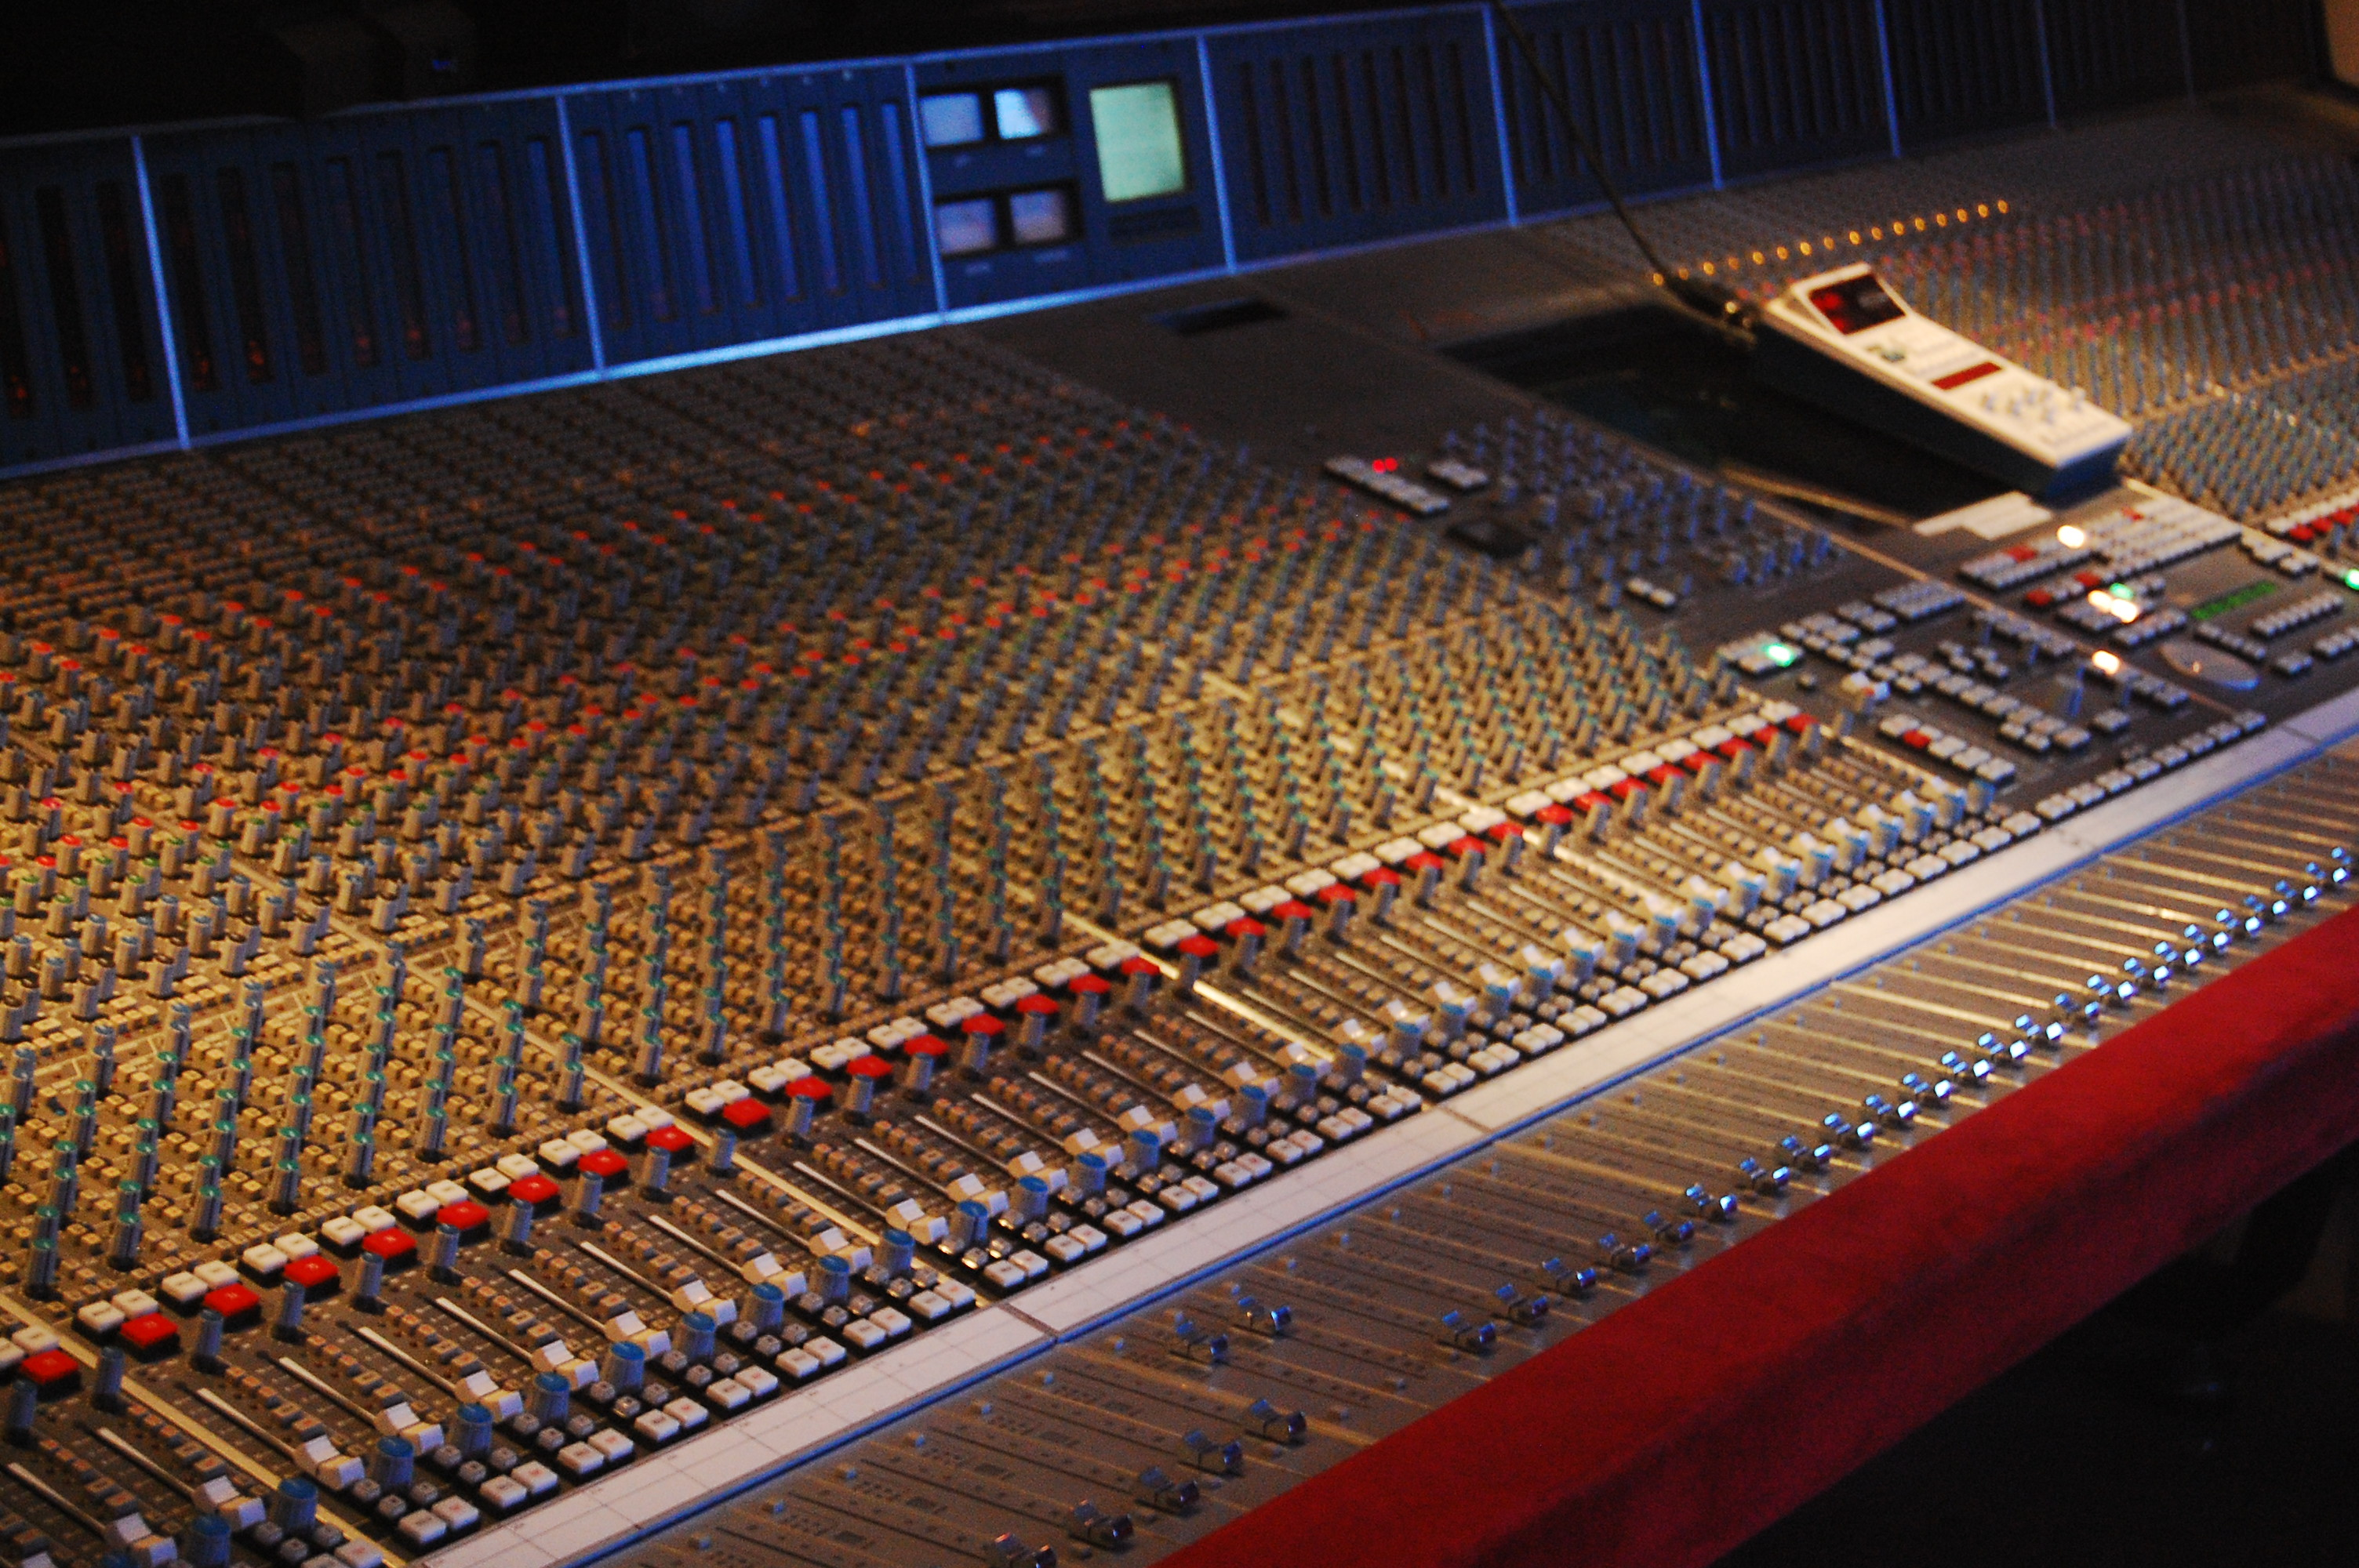
\includegraphics[width=0.8\textwidth]{./assets/ssl-hardware-mixer.jpg}
\caption{SSL SL9000J (72 channel) console at Cutting Room Recording Studio, NYC}
\label{fig:hardware-mixer}
\end{figure}
\label{org68040aa}
\end{LATEX}
The multi channel mixing desk metaphor is present in the large majority of DAWs
and is normally represented in a similar fashion to the sliders (or faders)
found in hardware mixing desks (see figure \ref{fig:hardware-mixer}). The mixing
desk enabled the producer to control the relative amplitude of a finite amount
of channels in addition to performing tasks such as panning to balance the
signal in a stereo field. The slim vertical sliders found on most systems were
codified in the 1960's by Bill Putnam \cite{bell_journal_2015}. This layout
allowed the producer to manipulate multiple channels of audio simultaneously in
a practice known variously as ``riding the faders'' and ``playing the mixer''.
Despite the fact that the digital variants of these are largely controlled by a
mouse that only affords the manipulation of a single fader at a time, they are
still, largely speaking, presented in this fashion on screen.

\section{Outboard effects unit}
\label{sec:orgf4bd48e}
\begin{LATEX}
\begin{figure}[h]
\centering
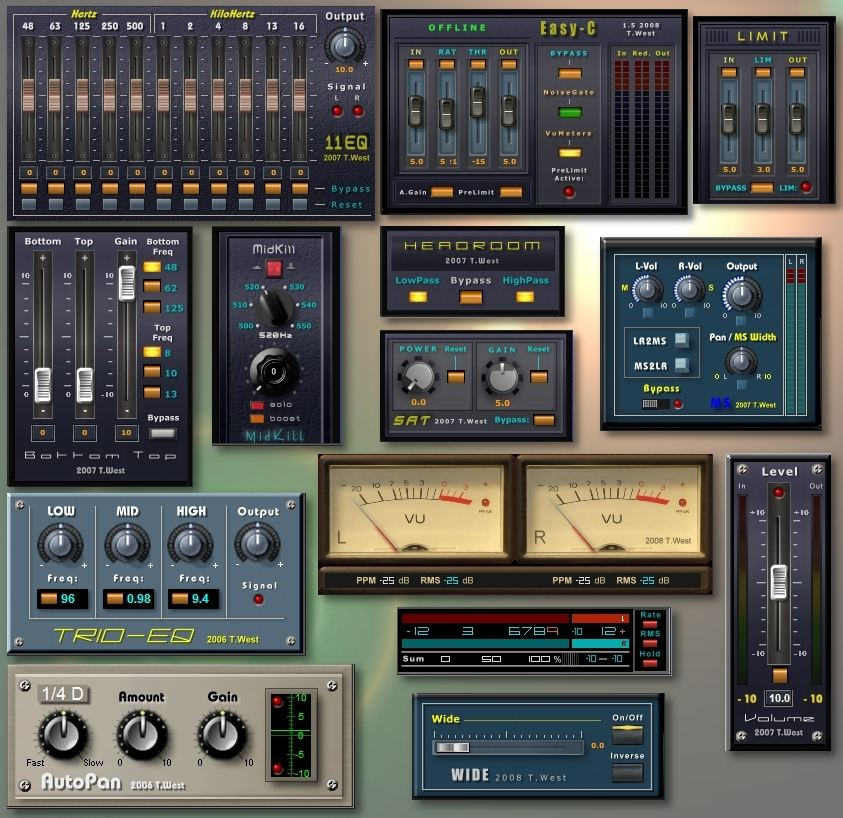
\includegraphics[width=0.6\textwidth]{./assets/fx.jpg}
\caption{Skeuomorphic software FX}
\label{fig:fx}
\end{figure}
\label{orgf63e9fb}
\end{LATEX}
Outboard effects are hardware units used in studios to add audio effects to one
or more channels on the mixing desk. The standard configuration of most studios
allows for two different ways of applying these effects, by using insert effects
and send effects. Insert effects are typically used when it only needs to affect
a single channel, for instance, a chorus effect applied on an electric guitar.
Send effects allow the producer to send a certain amount of the signal from a
channel to specialised channels to perform processing on the signal in parallel
with the original signal. It is typically used to apply effects on multiple
channels of audio such as reverb. The introduction of Virtual Studio Technology
(VST), by Steinberg, was responsible for bringing the outboard effects metaphor
to a whole new height. This allowed third party developers to create virtual
effects and instruments, and let producers expand their virtual studio beyond
the built in effects. The visual interfaces increasingly paid homage to their
hardware influences, emulating not only functionality but also the visual look
(see figure \ref{fig:fx}). \citet{levin_painterly_2000} describes this as
skeuomorphism, a design pattern where visual objects not only mimic real world
objects in functionality but also incorporate unneeded visual features. The
purpose of this is not only decorative but also educational, and gives
connotational cues as to how it should be used.

\section{The piano roll}
\label{sec:orgb8347d0}
The piano roll is a primary metaphor found in almost all mainstream DAWS and is
typically used to represent MIDI musical note information. MIDI, which stands
for Musical Instrument Digital Interface is a standard protocol developed in the
1980s to allow control instructions to be sent between devices. It provided a
standard language to for instance tell a synthesizer to play a particular note
at a precise time and duration. These instructions could be collected into a
MIDI file to, in effect, create a playable digital score. The piano roll is
slightly distinct from the previously discussed examples in that it originates
from a much earlier time period, the player pianos of the 1920s. The original
piano rolls were operated by feeding a roll of paper with holes punched to
indicate the precise timing that an attached piano should strike its notes. This
provides an apt and suitable description for the MIDI musical data it normally
represents. Similar to a player piano, no audible results are possible without
an attached piano, and in the case of MIDI, an attached sound generating
synthesizer device. \cite{bell_journal_2015,levin_painterly_2000}

\chapter{A compositional example}
\label{sec:org71fd778}
Rather than discussing the issues that can arise from the metaphors in the
abstract, let us consider a compositional idea and how we might achieve this in
a DAW. The idea is broken into the following compositional ``recipe'':
\begin{enumerate}
\item Two notes of the same timbre are played together about an octave apart for a
duration of 2 seconds.
\item The first note glissandos to the frequency of the second note and vice versa.
\item The first note starts with a small amount of vibrato that quickly dissipates.
\item The second note starts with no vibrato but adds a small amount as the note
nears completion.
\item When these two notes end, the same pattern is repeated except this time with
different timbres and frequencies.
\item This is repeated 3 more times with different timbres and frequencies to
complete this ten-second piece.
\end{enumerate}

While this may seem like a contrived example this, in fact, constitutes a
compositional technique called Klangfarbenmelodie that involves splitting a
melodic line between instruments or timbres to create a timbre melody. The
glissandos and altering of vibrato intensity add further complexity to better
illustrate some of the weaknesses inherent in DAW metaphors.

\section{Realization in a DAW}
\label{sec:org861cc88}
To achieve this in a DAW we have a few different options but a possible solution
would be as follows:
\begin{enumerate}
\item Working with the multitrack tape metaphor we can create ten separate tracks
to house two different versions of each timbre. A vibrato plugin effect
should be added to each of these by using a send or an insert effect. Two
different tracks are needed for each of the timbres due to the fact that the
two notes are played at the same time and both have different frequency and
effect trajectories. If on the other hand, they had the same effect
modulations or were played at different times, no additional tracks would be
needed.
\item Working with the piano roll metaphor, create a single note in each of these
tracks setting each one to the desired fundamental frequency.
\item Now edit the pitch bend automation lane by clicking into the relevant dialog
\item Similarly, open the relevant dialog to edit the intensity of the vibrato effect
\item Repeat this for each of the notes in the composition.
\end{enumerate}

At this point, we may have achieved what we set out to do. However, we now may
want to tweak each of these elements to taste and perhaps add more material. An
explosion in track count and overall complexity is inevitable. This can lead to
a serious slowdown in workflow, a loss of flow and cognitive overload. A common
technique to combat this complexity overload is to bounce the tracks and then
continue working on these simpler artifacts \cite{duignan_computer_2008}. This,
of course, negates a key advantage to working in a digital environment, the
fine-grained ability to freely change, tweak and undo. Locating each note in
separate tracks leads to an unnatural separation of what is, in fact, closely
related compositional material. This requires awkward context switching and
excessive navigation through the system to focus on different details.

There are of course other tools in the DAW that may achieve this task more
easily. For instance, a sampler may allow us to use different timbres on the
same track and may work better in this case. We now have the extra task of
exporting each of these samples in preparation for our composition work. Some
other options present in many DAWS include aggregate instruments, multi-timbral
instruments, and perhaps some midi routing options. Another option is to use an
alternative, more flexible, environment such as an audio programming language.
Some brief consideration of this will now be given.

\section{Realisation in code}
\label{sec:org64567ed}
The piece could be realised in quite a straightforward manner in an audio
programming language such as \emph{Csound}. Central to \emph{Csound} is the concept of the
\emph{unit generator} (or ugen), an abstraction to define both sound generators and
processors. These can be patched together in a simple textual coding language to
form instruments. A score is then specified, again in code, to define note
onsets, durations in addition to other arbitrary parameters defined in the
instruments. Each of the required timbres could have been represented as
separate csound instruments, with each one configured with the desired timbre in
addition to the vibrato effect. \emph{Function tables} could be used to control the
movement of the pitch glissando and the varying vibrato intensity. A function
table is a list of numbers in Csound that can be read from, at various speeds,
to supply control data to parameters (amongst other uses). A number of routines
are available in Csound to generate commonly used list types. In this case, a
line segment generator would be most applicable and would be used to generate a
shape such as shown in fig:gen05. The Csound score would refer to each of the
defined instruments with each note amounting to a single line of code, making
the entire score a total of five lines. Demonstration code is provided in the
appendix.

Depending on the experience of the reader, this may or may not seem like a
better approach than using the DAW owing to the following central issue. It is
not beginner friendly and a reasonable amount of prior experience and/or
training is required. Perhaps a bigger criticism that could be made, however, is
that it can lead to an analytical rather than a creative way of thinking. In
``Thinking Slow, Acting Fast'', Daniel Daniel Kahneman contrasts these two ways of
thinking which he terms \emph{System 1} and \emph{System 2}. System 1 is instinctive,
fast, emotional and is a mode of thinking that may not register consciously.
System 2 is slow, logical, analytical and registers prominently in active
consciousness. Routine tasks such as walking, opening doors etc only use system
1 thinking. These can be completed while exerting minimal cognitive effort (all
the while calculating the complex motor sensory actions that must take place).
Complex analytical tasks such as programming require system 2 thinking.
Approaching creative tasks such as music making in this way where instinct and
emotion are often crucial can slow down or stop the process. Perhaps it is best
summed by John Cage: ``Don't try to create and analyse at the same time. They're
different processes'' \cite{popova_10_2012}.

\chapter{Sketching as an alternative metaphor}
\label{sec:orgb0109e3}
While audio programming languages offer a model that is closer to the underlying
computational processes taking place than the more abstracted DAW interfaces. As
we have discussed, though what is gained in flexibility can be lost in
intuitiveness and ease of interaction. Rather than discarding these higher level
metaphors, perhaps a better approach would be to explore alternate metaphors.

A rather promising but nonmainstream approach is that of sonic sketching. This
has a long and illustrious historical precedent reaching back well before the,
now more prevalent, studio metaphors. Graphical sound generation techniques have
a long history starting with experiments beginning in the early 20th century
\cite[pg. 329]{roads_computer_1996}. The technique of the optical soundtrack,
however, brought these ideas to a new level of sophistication. The technique,
which involved placing marks via photography or direct manipulation to specify
audio properties, was explored by such luminaries as Oskar Fischinger, Norman
McLaren and Daphne Oram. Oram's particular take on the technique will now be
discussed.

\section{Oramics}
\label{sec:orgd7f5284}
A primary motivating factor behind Daphne Oram's development of the Oramics
machine was to bring more human-like qualities to the sounds generated by
electronic means. The machine worked by playing back multiple lanes of film tape
in unison, defining a monophonic series of notes as well as control signals to
shape their timbre, pitch and amplitude. She details the thought process behind
this in her journal style book, ``An Individual Note''
\cite{oram_individual_1972}.

The aspects of the sound that she wishes to control are volume, duration,
timbre, pitch, vibrato, and reverb. In order to do this, she describes a simple
musical notation language based on the freehand drawing of lines combined with
discrete symbols. The lines, which she describes as the analog control, are used
to define volume envelopes. Interestingly, the default and preferred method for
the parameters she wishes to control is the continuous line rather than discrete
note symbols. For instance, she avoids the use of a static velocity per note and
instead only specifies the use of a control envelope to change amplitude.

The discrete symbols, which she categorizes as digital control, are used to
define individual pitches and are termed neumes. She highlights that notes
should not remain static and, thusly, an analog control of each note is also
specified. Similarly to amplitude and vibrato, timbre is also defined by the
freehand drawing of lines and is something that with practice the ``inner ear''
can develop an intuition as the sonic results of different line shapes. It is
Oram's belief that the hand drawn nature of the lines make the results slightly
inaccurate and to some extent unpredictable. Herein, however, lies the
possibility of bringing more humanity to the cold and precise machines
generating the electronic signal.

\section{UPIC}
\label{sec:org3e2e8ed}
\begin{LATEX}
\begin{figure}[h]
\centering
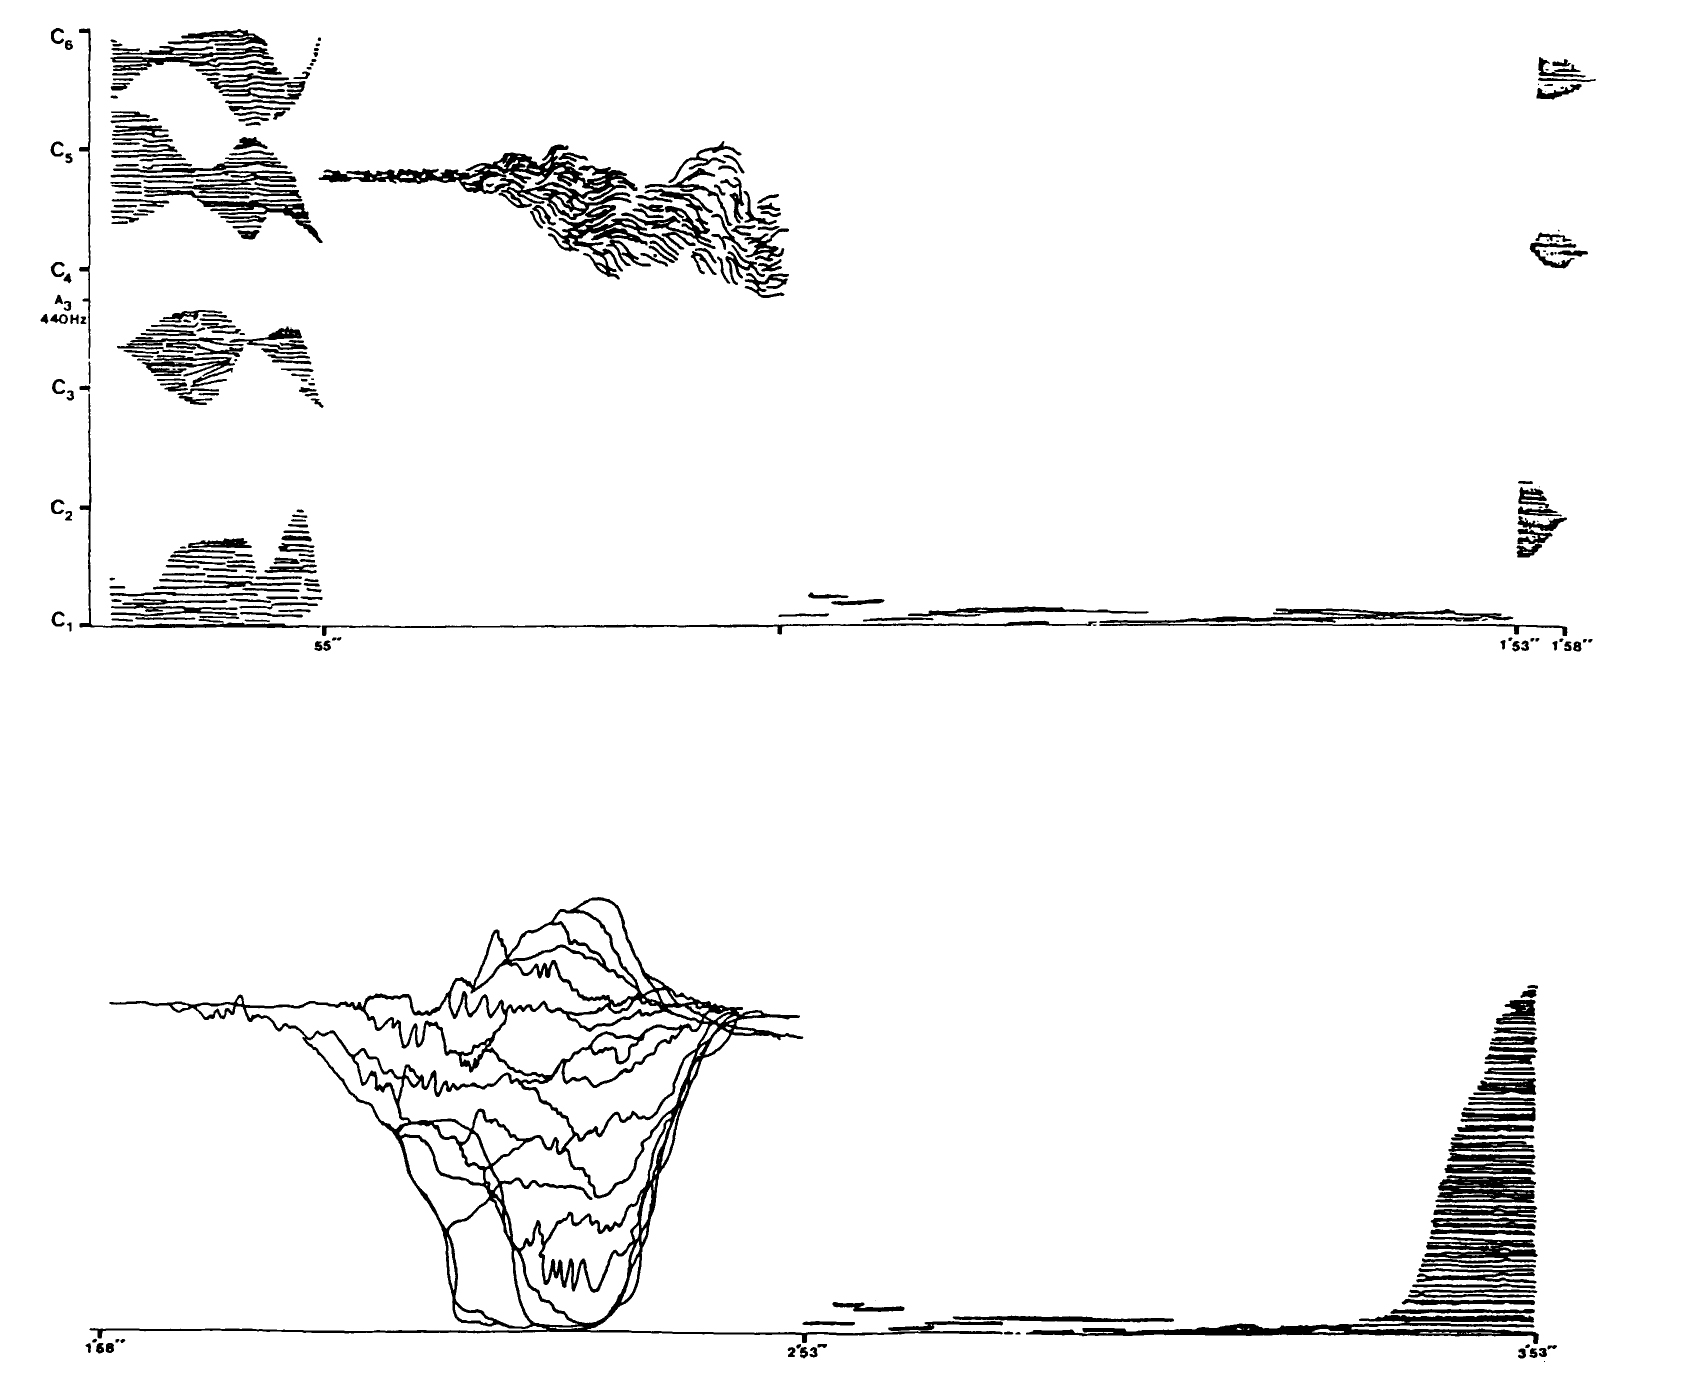
\includegraphics[width=1.0\textwidth]{./assets/Iannis-Xenakis-Mycenae-Alpha-score.jpg}
\caption{Iannis Xenakis - Mycenae Alpha score}
\label{fig:xenakis-alpha}
\end{figure}

\begin{figure}[h]
\centering
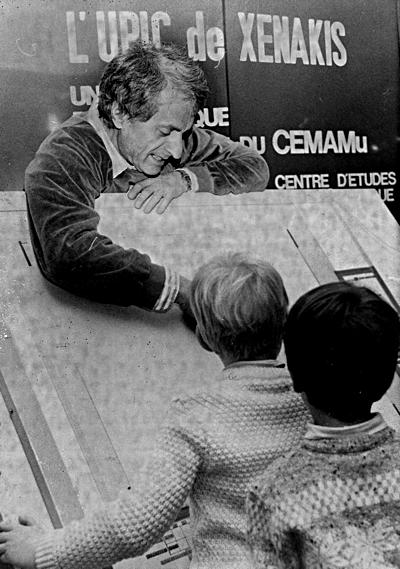
\includegraphics[width=0.5\textwidth]{./assets/xenakis-and-the-upic-system.jpg}
\caption{Iannis Xenakis showing UPIC to a younger audience}
\label{fig:xenakis-children}
\end{figure}
\label{orgbdc8b3c}
\end{LATEX}
The UPIC (``Unité polyagogique informatique du CEMAMU'') was a graphic sound
synthesis system that was designed by Iannis Xenakis and arose from his graphic
approach to composition. His earliest work, ``Metastasis'', was conceived using a
graphic approach to describe the trajectories and sound masses that inhabits the
orchestral landscape of the piece. This approach has been attributed to his
background in architecture, having worked in the studio of Le Corbusier. The
UPIC was first conceived of in the seventies with the realisation of the first
version in 1975 and its first public showcase in 1977 \cite[pg.
331]\{roads\_computer\_1996\}. The work ``Mycanae Alpha'' (figure
\ref{fig:xenakis-alpha}), composed in 1978 was the first work to use the system
and was a ``nine-minute 38-second composition of dense and intense textures, of
phase-shifting waveforms rich in harmonics that cascade, flutter, crash, and
scream like sirens in a vast cosmological territory''
\cite{tyranny_mycenae-alpha_2017} .

The early version of the UPIC worked by drawing on a large digitizing graphics
tablet which was interpreted by a high-powered computer (for that period) and
converted into audio signals. The graphic approach to sound specification worked
on a synthesis level by allowing the composer to draw and audition waveforms.
Larger structures could be drawn in by switching to a ``score'' page and drawing
lines, or ``arcs'' as they were denoted, on a pitch-time canvas. The final version
of the application ran on personal computers and allowed for real-time
interaction with a 64 oscillator synthesizer. At this stage, the input means had
changed to a computer mouse but nevertheless retained the graphic approach of
interaction. \cite{nunzio_upic_2014}

A primary goal of the UPIC project was that of pedagogy. Xenakis reasoned that
the universality of sketching meant that it could provide an excellent teaching
tool for a wide audience, even for young children (figure
\ref{fig:xenakis-children}). Another goal of the system was to encourage
composer autonomy. At the time of its conception in the seventies, the technical
barrier to entry into electronic music creation was very high and interfaces to
help with this were rare or non-existent. Though the UPIC is not available to
the general public currently, it has inspired a number of other systems that are
available today.  \cite{nunzio_upic_2014}

\section{A Golan Levin's AVES}
\label{sec:orgaf7560a}
Golan Levin created the interactive audio-visual system, AVES, a series of audio
visual installations in the late nineties and represented a landmark in the
field of visual music. It is an attempt to move away from the diagrammatic
approach to musical interfaces and to present an interface that is painterly in
approach. Taking strong influence from visual artists such as Paul Klee, he
presents a system that maps user input from a graphics tablet and mouse to
visuals and audio. The intention is to create a strong visual correlation
between these two modalities. A variety of approaches are taken to achieve this,
all of them involving an algorithmic approach to a certain degree. For instance,
in the piece ``Aurora'', he maps visuals of vast quantities of particles to a
granulated sound synth sound source. He didn't take the approach of an exact
mapping of visual particles to audio particles, however, and instead used a
statistical control approach to approximate the correlation in between the
visual and aural. \cite{levin_painterly_2000}

For Levin, the digital pen input in combination with it's infinite variability
represents an ideal instrument for creative expression in his digital temporal
audio visual paintings. \cite{levin_painterly_2000} The reason he gives for this
is, similar to a musical instrument such as a violin, the pen is instantly
knowable in that a child can pick it up and start creating marks but infinitely
masterable through practice and hard work, and ultimately a vehicle for creative
expression after a certain amount of mastery. A set of criteria that he and John
Maeda arrived at to evaluate the success of their experiments was: is it
instantly knowable, how long did you use it, how much of your personality can be
expressed through it and, finally, with practice is it possible to improve using
it.

Levin's work is largely realtime and transitory in nature with gestures giving
rise to visual and audio reactions that rise, fall and dissipate. A description
that he uses of some of work is that of creating ripples in a pond. Therefore
his work is very much geared towards an instrument like experience. It is not
concerned with the recording or visualization of a score or timeline of musical
events as would be the function of a compositional tools such as a DAW. Indeed
it is a conscious design decision to avoid such representations. Many of the
principles and ideas of his work can, however, be applied in the context of a
composition tool.


\section{William Coleman's sonicPainter}
\label{sec:orgc177a72}
\begin{LATEX}
\begin{figure}[h]
\centering
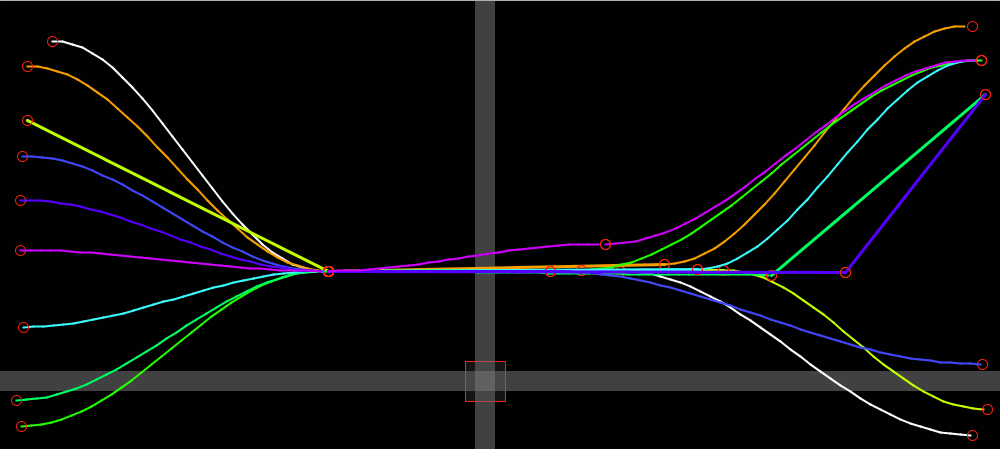
\includegraphics[width=1.0\textwidth]{./assets/sonicpainter2.png}
\caption{SonicPainter by William Coleman}
\label{fig:sonicpainter}
\end{figure}
\label{orgad9164a}
\end{LATEX}
SonicPainter by William Coleman is a novel musical sequencer that seeks to
address some of the shortcomings of traditional approaches to music sequencing
found in commercial DAWs \cite{coleman_sonicpainter:_2015}. The focus of the
line and node based interface (see figure \ref{fig:sonicpainter}) is to bring
timbral shaping to the fore rather than being hidden away in miscellaneous
automation lanes. The design takes influence from legacy musical systems, in
particular, the UPIC and incorporates ideas from visual music and embodied
cognition.

Similarly to traditional sequencers, the x axis represents time and the y-axis,
pitch. Note information is input via keyboard and mouse. A click starts a note
and can be followed with additional clicks to continue to shape it. It can be
ended by clicking a keyboard shortcut. By drawing notes as lines in this manner,
the unfolding of the note can be explicitly represented visually. Other timbral
aspects such as vibrato are represented by further visual manipulation of the
line. For instance, an overlaid sine wave line indicates the timing and
amplitude of the vibrato. In addition, the system allows for freehand input of
notes. 

\chapter{Conclusion}
\label{sec:org9f3a411}
The dominant metaphors present in DAWs, which are by and large analog studio
influenced were discussed including details on their origins and their
reincarnation in digital form. A short compositional example was given and the
process to realise this in a DAW was described. The piano roll, multi-track
mixer, and outboard effects metaphors were shown to be a poor fit for this
particular compositional idea and resulted in an excessive amount of tracks and,
therefore, complexity. A simpler solution was described in the csound audio
programming environment. The lower level abstractions provided here allowed for
a more succinct and simpler implementation of the piece. Some potential pitfalls
to this approach were given. This includes a steep learning curve for novice
users and a potential bias towards an analytical rather than a creative mode of
thinking. Rather than abandoning the high-level metaphors present in DAWs it was
posited that another approach could be to explore other metaphors more suited to
certain compositional ideas. To this end, the metaphor of sketching as an
interface to audio systems was explored by tracing it's early roots in the
optical soundtracks of Oram to the realtime synth sketching of Xenakis's UPIC
through to the contemporary approaches of Golan Levin's AVES system and William
Coleman's SonicPainter.

\newpage
\part{Methodology}
\label{sec:org30c50d3}
\chapter{Introduction}
\label{sec:org333e3b4}
This chapter outlines the approach that will be taken in the realisation of the
SonicSketch application. An assessment of SonicPainter will be given to identify
the features that will be incorporated, improved on or omitted. The major
technologies being used in the project will then be introduced along with some
justifications for their usage. These include the \emph{Web Audio API}, \emph{Tone.js},
\emph{Paper.js}, \emph{ClojureScript} and Facebook's \emph{React} framework.

\chapter{Assessment of SonicPainter}
\label{sec:orgcb78f75}
As has been mentioned previously, the SonicPainter application developed by
William Coleman will form the basis of the work on SonicSketch. While the basic
design of SonicPainter works very well and is aligned with the goals of
SonicSketch in the following ways:
\begin{itemize}
\item Provides a simple immersive score space that represents time on the x-axis and frequency on the y-axis.
\item Allows multiple voices or timbres to be represented in this space so that all
notes can be seen at a glance without having to click into separate tracks.
\end{itemize}
\begin{itemize}
\item Visualisation of vibrato effect using overlaid sine wave is suitable in theory
but perhaps could be implemented better.
\begin{itemize}
\item Uses FM synthesis as the synthesis engine. This versatile and efficient is a
good fit particularly for use in the web browser where performance can be an
issue.
\end{itemize}
\end{itemize}
Some issues that have been identified with SonicPainter will now be addressed.
It should be noted that as the software is only at a prototype stage some of the
shortcomings outlined here may not be design decisions and instead may be
implementation issues.

\section{Usability issues}
\label{sec:org7cf97ca}
While the application is conceptually straightforward and beginner friendly
there are some stumbling blocks that would make it difficult for a new user to
begin using it. Starting a note is obvious and involves simply clicking on the
screen to anchor the start point. A line now becomes attached to from this point
to the mouse pointer location, indicating that another press will finish the
note. However, this instead adds a point to the note, indicated by the fact that
a new line appears between this new point and the pointer position. It is
unclear how to finalise the note. The solution is to press the \textbf{shift} modifier
key and click. Some simple labeling could alleviate this issue, by perhaps using
a small toggleable information box. Unfortunately, this issue repeats itself in
a good deal of the functionality with additional features hidden behind keyboard
shortcuts that would be difficult or impossible to discover.

\section{Issues with audio visual connection}
\label{sec:org52e03e7}
Some deficiencies were found with the mapping between visuals and audio. It is
possible to draw multiple concurrent notes that share the same timbre suggesting
that the audio would polyphonically sound the notes together. This is not the
case however and only one note can be played back at the same from the same
timbre. To achieve this, a separate voice must be used by clicking the up arrow.
To remedy this issue, it could either prevent the creation of concurrent notes
visually or allow multiple notes to sound together by making each voice
polyphonic.

\section{Invalid states}
\label{sec:org9d9edf9}
A serious technical issue with SonicPainter is the presence of invalid
application states that are not properly handled in the code. These arise when
the user performs a series of actions that are not properly handled either by
catering for them or by disallowing them. An example of this is when the user
starts a note and then changes mode to, for instance, vibrato. When this
happens, the application allows the mode to change and carry out the vibrato
change all the while keeping a line connected to the pointer position. From here
it is not possible to complete the note without returning to the original mode
and clicking multiple times.

This unexpected behaviour could be avoided by either disallowing mode changes
during note creation or by ending the note when the mode has changed. These type
of issues are common even in commercial applications as is illustrated in Harel
(???). An example he gives is that of a calculator built by Microsoft that
enters an invalid state in a number of different situations. To counter these
issues a disciplined approach will be taken to managing state in SonicSketch by
performing \emph{validation} operations and the use of \emph{finite-state Machines} (FSM).
Validation is a technique used to ensure that data is in the correct format and
that any required information is present and in an allowable format. A
finite-state machine is a computational model that can be in only one of a
finite number of states. These states may change due to external input which
triggers transitions from one state to the next. They can prove useful in
avoiding invalid states and to reduce the amount of conditional logic in the
program.

\section{Linear representation of frequency}
\label{sec:org262933f}
The SonicPainter represents a frequency range of 20-500 Hertz (Hz) on its
Y-axis. This is mapped linearly from the on-screen coordinates to frequency
values. It is not made clear why this range and mapping was chosen and may have
been for aesthetic reasons. Psychoacoustically it may be suitable to map this
linearly as this corresponds to the linear perception of frequency at the lower
frequencies. This phenomenon is represented in the Bark Scale, which is a
psychoacoustic frequency scale on which equal distances correspond to
perceptually equal distances. However, the range of 20-500 Hz frequency is quite
limiting given that the highest note of a piano can reach to 4186 Hz. In
addition, there is a strong cultural expectation of logarithmic mapping of
frequency owing to the semitone being a logarithmic scale.

\chapter{Technical approach}
\label{sec:orgd79ead1}
\section{Audio in the modern Web Browser}
\label{sec:org812b131}
The W3C Web Audio API specification allows audio processing to take place in the
web browser. Audio generation and processing is defined using an \texttt{AudioContext}
graph of connected \texttt{AudioNode} objects. While javascript processing is supported
(by using a \texttt{ScriptProcessorNode} object), most processing takes place in
optimized lower level languages such as C or C++. Advanced synthesis techniques
are possible by connecting audio generating nodes to processing nodes. Audio
generating nodes include the \texttt{OscillatorNode} to generate a periodic waveform
and the \texttt{AudioBuffer} to playback audio waveforms. Processing nodes include the
\texttt{GainNode} to adjust the amplitude of a signal and \texttt{BiquadFilterNode} filter the
signal. Parameters of these nodes may be adjusted smoothly over time using the
\texttt{AudioParam} interface to, for instance, slowly fade a synth sound in.

\section{Tone.js}
\label{sec:org0a3276a}
Tone.js is a Web Audio framework that provides several helpful abstractions and
libraries to help interaction with the Web Audio API. A central aim of Tone.js
is to enable some of the conveniences of DAWs and is formed on three tenets:
musicality, modularity, and synchronization. An example of this is the
flexibility it allows to express time values, eg. ``\texttt{4n}'' for a quarter note in
metrical notation, \texttt{1} for a second and ``\texttt{100hz}'' to express 100 hertz, etc.
These are all converted to seconds before scheduling them with the Web Audio
API. A system called ``just in time scheduling'' ensures that tempo-relative
values are not scheduled until the latest possible moment, thus ensuring that
they reflect the latest tempo value.

The primary reason that Tone.js was chosen was for the signal system that it
uses to make working with parameter modulation easier and more efficient than
working directly with Web Audio API. This uses a constant signal generator
running at audio rate connected to a GainNode. In addition, this value can be
multiplied and summed using GainNodes native capabilities enabling performant
signal processing operations on all parameters. For instance, \emph{FM synthesis}
generally requires that a relative relationship is maintained between the two
oscillators, the carrier, and the modulator. When directly using the Web Audio
API Param, a \texttt{ScriptProcessorNode} would need to be setup to calculate this
which is not as efficient or as straightforward as carrying out the calculations
using Tone.js signals.

\section{Paper.js}
\label{sec:orge9fdc1a}
Paper.js is a descendant of Scriptographer, a scripting tool for Adobe
Illustrator a vector graphics program. It runs in the web browser canvas
element, running in its 2d mode. Paper.js adds a number of features to the
browsers native canvas element including a \emph{scene graph}, geometry and vector
abstractions as well as tools to draw and animate shapes on-screen. The central
abstraction in Paper.js and any vector system is the \emph{path}. This allows for the
specification of any shape by describing start points and endpoints for a series
of paths. Curves can be added to these paths by adjusting an additional set of
points associated with a path, the \texttt{handleIn} and \texttt{handleOut} points. These
define control handles that alter the curvature of the line using Bezier
mathematics.

A primary reason that Paper.js was chosen for SonicSketch is the path
simplification algorithm that allows the data captured with freehand input to be
simplified and smoothed. Instead of just plotting every point captured, an
optimized subset of these points is used to reduce memory usage and speed up
drawing. It is based on an algorithm by Philip J. Schneider published in
Graphics Gems (1990). In addition, these simplified paths are more suited to
mapping to control data for the audio system.

\section{React framework}
\label{sec:org3290054}
\emph{React} is a web framework built by Facebook that aids the developer in updating
the document object model (DOM), a process that is required when the state of
the application changes. This was a role traditionally carried out by the web
server and delivered to users as a static page. This saw a significant change
however with the rise of single page applications (SPA) around 2010. The
advantage of the SPA is increased interactivity and responsiveness to user
input, allowing the look and contents of the page to update dynamically as the
user interacts with the webpage. To aid in the construction of these SPA's a
number of frameworks to help the process were introduced by the open-source
community. Some popular early examples include Backbone.js and Angular.js. A
technique that saw some popularity was a system called two-way binding which
created a two-way link between the current state in the model and the visual
appearance of the view. This, however, has a number of issues including some
serious performance issues, in addition to some conceptual problems
\cite{whelpley_is_2014}.

React offers a simpler one-way binding system using what is termed the \emph{virtual
DOM}. This works by maintaining a virtual version of the dom in a javascript.
When the virtual DOM changes, the parts of the real DOM that require changing
can thusly be pinpointed and efficiently updated. This system has proven to be
particularly beneficial when paired with \emph{functional programming} techniques, a
style of programming that encourages the use of pure functions as the primary
building block of programs. In the case of working with the DOM, it can lead to
not only an increase in efficiency in the rendering of the applications but also
a simplification of the programming model as a secondary benefit. A number of
projects have emerged that attempt to bring this secondary benefit beyond the
realm of the DOM. This includes writing command-line programs
\cite{demedes_vadimdemedes/ink:_2017}, writing web audio applications
\cite{formidablelabs_react-music:_2017} and even for embedded electronics
\cite{kasten_react-hardware:_2017}.

\section{Clojurescript}
\label{sec:org3a005d7}
Clojurescript is a compile to javascript programming language that is based on
Clojure, a modern \emph{Lisp} that runs on the Java virtual machine. Lisp is a
programming language that was invented by John McCartney in the 1960's and is
known for its minimal syntax consisting primarily of parens. The word Lisp is
derived from the term ``List Processor'' as Lisps source code and data structures
are built around lists. Clojure and ClojureScript promote a functional
programming style. Clojurescript and other functional programming languages such
as Elm have seen an increase in usage in the past number of years as this
paradigm has proved useful in managing complex stateful UIs. Some annotated
examples of ClojureScript follow that show the basic building blocks of the
language and will help in understanding the code walkthrough in the next
chapter.

\begin{footnotesize}
\begin{verbatim}
;; A list. It is quoted as otherwise it would treat it as a function call
'(1 2 3 4)

;; Call a function. In this case calling the multiply function.
(* 2 2)

;; Define a variable a
(def a 1)

;; Define a function b
(defn b [n] (* n n))

;; A vector is the most common way to represent sequential data in clojurescript
[1 2 3 4]

;; A hashmap is used for associative data and more often than not uses keywords
;; as keys. Keywords are used similarly to constant strings in other languages.
{:hello "world"}

;; Vectors and hashmaps are immutable and can't be changed after they've been created
;; An atom is used for data that needs to change (to model state changes for instance).
(def c (atom 1))

;; To change it's value use the reset! function.
;; Here it changes the c atom to 2.
(reset! c 2)

;; Clojurescript can interface with javascript in a straightforward manner
;; but uses a slightly different syntax. The term that is normally
;; used to describe this is js interop.
;; Calling a function:
(js/console.log "Hello world")
;; Calling a method on an object:
(.reload js/location)

\end{verbatim}
\end{footnotesize}

This covers some basics that will be particularly helpful for readers that are
familiar with C style languages. A more in depth is beyond the scope of this
document and interested readers should consult the many resources available
online. The most commonly used build tool that is used with ClojureScript (and
Clojure) is \emph{Leiningen}, which takes care of managing the code dependencies and
converting the code from ClojureScript to javascript. These dependencies are
defined in the ``project.clj'' file. The primary dependencies used by SonicSketch,
\emph{Reagent} and \emph{re-frame} will now be discussed.

\section{Reagent \& Re-frame}
\label{sec:orgd633c6c}
Reagent is a library that provides an idiomatic ClojureScript interface to
React, allowing ClojureScript to harness the DOM manipulation facilities
provided by React. This delegates the \emph{side-effects} of rendering and
manipulating DOM to React's reconciler algorithm. Side-effects is a functional
programming term to denote anything that isn't related to the supplied arguments
or return value of a function. This is normally object mutation (to change the
state of the program) or input/output (I/O) operations, e.g. writing a file to
disk, displaying graphics or playing a sound. \cite{sylwester_meaning_2015} In
addition to the interface to React, it provides a special reactive atom that
efficiently re-renders React components when the state changes.

Re-frame is a framework that uses Reagent's interface to React to manage views
and it's reactive atom to manage state. It proposes a program architecture
consisting of the following 6 elements:
\begin{enumerate}
\item Event dispatch
\item Event handling
\item Effect handling
\item Query
\item View
\item DOM
\end{enumerate}
The majority of events that are dispatched are due to user interactions with the
system (for instance on a mouse click). Event handling is the code that is run
in response to these events. Re-frame submits that these event handlers should
supply data to describe the side-effects rather than carrying them out in the
handlers. Re-frame carries out this work which is typically to update the
application state. This is stored in a single reactive atom and managed by the
framework. A subscription system allows the view system to update when the state
that it depends on changes. Finally, React updates the DOM to complete the
cycle.

\chapter{Conclusion}
\label{sec:orge44d228}
SonicPainter was discussed in some depth with a focus on issues that will be
improved on in SonicSketch. The technologies being used in the SonicSketch app
were described in detail including some brief justification behind these
technical choices. This covered the Web Audio API technology that underlies the
audio aspect of the project, as well as the libraries and frameworks being used
to manage the views and state of the app.

\newpage

\part{Execution}
\label{sec:org36d7499}
\chapter{Introduction}
\label{sec:orgca7b8ad}
The following chapter gives an outline of the process that was undertaken to
build out the final application. A description of early prototype work is given
to give context to the construction of the final working prototype version. This
is followed by a description of the technical architecture of the system as well
as an outline of the sometimes difficult setup process of getting the various
architectural elements working together. A detailed discussion of the core
functionality of the system is then given, followed by a description of
functionality that is more secondary in nature.

\chapter{Early prototype work}
\label{sec:orge7f5328}
\section{MelodyPainter}
\label{sec:org890ff4f}
\begin{LATEX}
\begin{figure}[h]
\centering
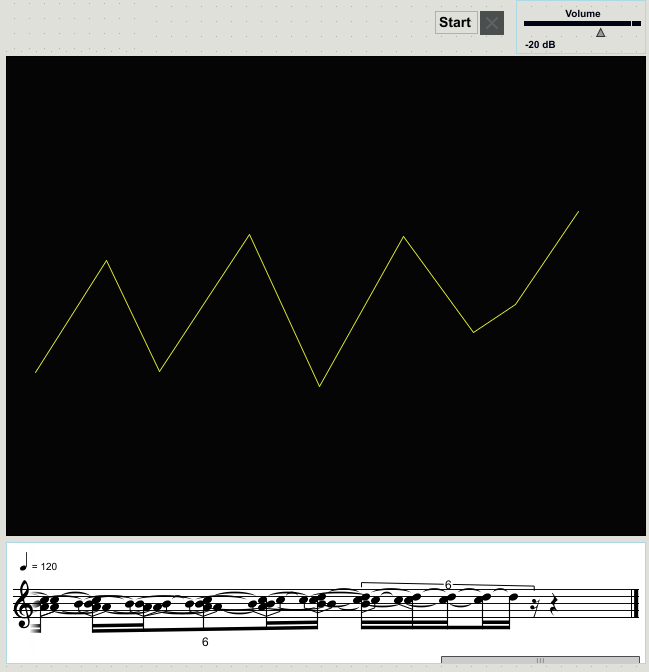
\includegraphics[width=0.65\textwidth]{./assets/melodysketch.png}
\caption{MelodySketch interface}
\label{fig:melodysketch}
\end{figure}
\label{orgaa063c0}
\end{LATEX}
MelodyPainter is an early protoype built out in Max MSP that allows users to
draw freehand lines, which are converted into break point function data and used
to generate a melodic profiles using Bach for Max MSP \cite{agostini_max_2015}.
Bach is a suite of composition tools that allow for a number of computer aided
composition techniques (CAC) and provides similar functionality to IRCAM's Open
Music system. These melodic profiles are then filtered to only includes notes
from a pentatonic scale, to give reasonably pleasing aural results. Some notable
flaws in the system include the following. It is limited to strictly western
tonal music styles. It has no allowance for rhythm and plays only eight notes
giving results a noticeably bland and predictable quality. The freeform nature
of sketched input however was quite a pleasing means of inputting the control
information.

\section{SonicShaper}
\label{sec:org3b9936f}
\begin{LATEX}
\begin{figure}[h]
\centering
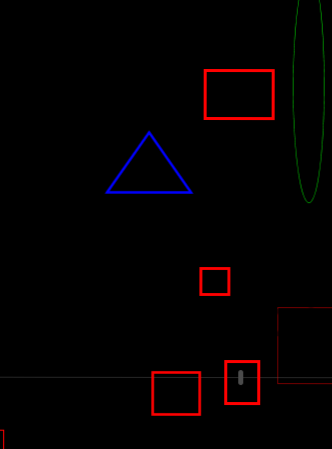
\includegraphics[width=0.4\textwidth]{./assets/ss.png}
\caption{SonicShaper interface}
\label{fig:sonicshaper}
\end{figure}
\label{org5ebb57c}
\end{LATEX}
A separate application was created in Processing which allowed users to draw
shapes, using either mouse or ideally, pen input. A sound that is associated
with each shape is then played back. As the sound of each shape plays back, it
is lit up using animation, creating a strong connection between the shape and
it's resulting sound. The application uses the ``gesture variation follower''
system \cite{caramiaux_adaptive_2015}, which while promising in principle, didn't
have a high rate of accuracy in recognizing the shapes.

\section{Web version of William Coleman's SonicPainter}
\label{sec:orgc437744}
\begin{LATEX}
\begin{figure}[h]
\centering
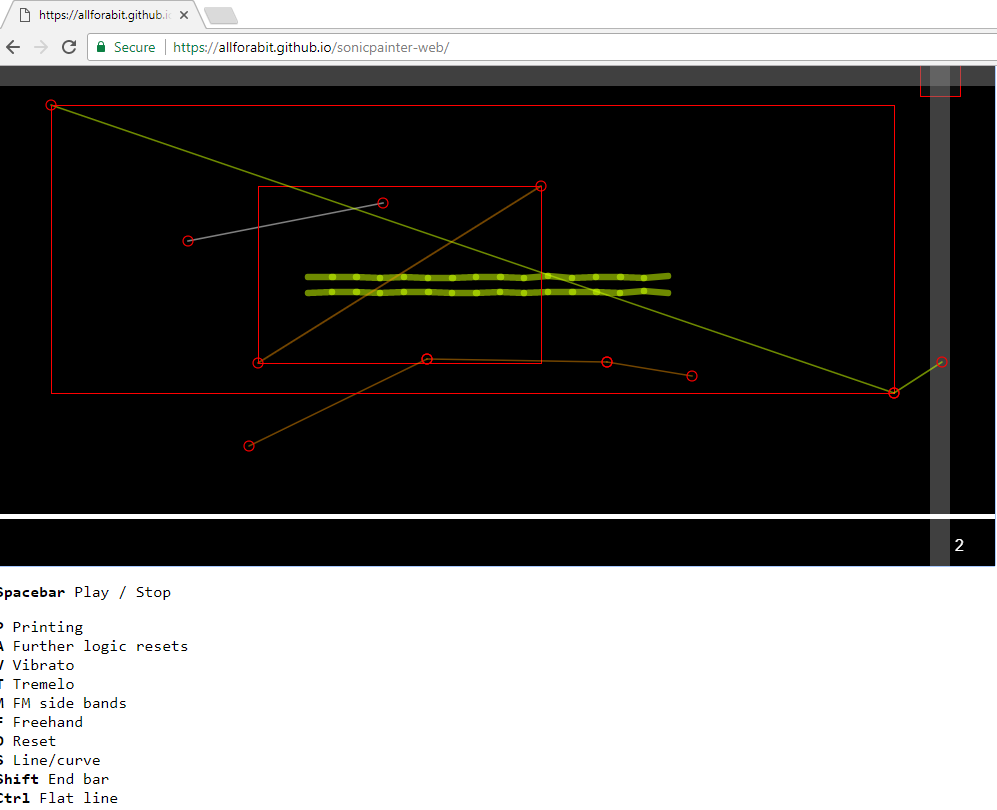
\includegraphics[width=1.0\textwidth]{./assets/sonicpainter-web.png}
\caption{SonicPainter in a web browser}
\label{fig:sonicpainter-web}
\end{figure}
\label{org7d979bf}
\end{LATEX}
A potential starting point that was considered was using the code from William's
SonicPainter and porting it to the web browser
\cite{coleman_sonicpainter:_2015}. This process proved to be quite
straightforward. The processing code could be embedded in a webpage with minimal
modification, using ``processing.js'', a web version of the Processing library
that enables users to run processing sketches in the Web Browser
\cite{fry_processing.js_2017}. Some notable changes that had to be made were
removing the OSC functionality as this is not technically possible to use in a
browser. In addition, some other pieces of code were removed and altered
slightly. As it's not possible to run Max MSP patches in the browser, the audio
system was re-implemented using Tone.js \cite{mann_interactive_2015}. As
SonicPainter uses simple FM synthesis, a very close approximation to the
original version could be created. In the end, it was decided not to build on
this codebase however due to the issues with functionality and usability
detailed earlier. These would be difficult to resolve in an inherited codebase.
The process of porting the code did however give a more in depth incite into
Coleman's implementation. 

\chapter{Setting up the architecture}
\label{sec:orgb644dd8}
\section{Clojurescript and javascript npm modules}
\label{sec:orgdd0bac0}
Despite the fact that clojurescript has existed for six years
\cite{sierra_clojure_2011}, some areas of the development process are still
difficult, particularly when building out a more complex real world
applications. It should be noted that a good deal of work is being carried out
to make this a smoother experience and, thusly, it is likely to become easier in
the near future \cite{monteiro_clojurescript_2017}. It should also be noted that
building applicatons using plain javascript is not a trivial process either and
in will , in all likelihood, include a complex build process using a system like
webpack or browserify.

A primary issue that had to be resolved to allow the application development to
proceed was the incorporation of javascript npm modules. NPM is the package
manager used by \emph{node.js}. Node.js is a javascript platform originally designed
for more server oriented applications, but, increasingly, also for rich
client-side applications. The related NPM repository houses a large amount of
javascript packages (currently 477,000) and is one of largest collections of
code in the world . For a pure javascript application, it would be a matter of
simply adding the desired libraries as NPM dependencies. However, with the use
of ClojureScript, some extra steps needed to be carried out. In addition to
adding these dependencies, a javascript file needed to be created that imported
these into a \texttt{deps} object. This \texttt{deps} object could then be referred to in
ClojureScript using the standard interop syntax \texttt{js/deps.myDependency}
\cite{weller_clojurescript/reagent_2017}. At the time of development, an alpha
feature that allowed npm dependencies to be declared as part of the project.clj
file was experimented with but was not used due to some implementation
difficulties. While the project setup was not as elegant or succinct as might be
wished, it did provide a stable base to build on. Crucially the rich resource
that is the NPM ecosystem could now be harnessed, to use such tools as Paper.js
and React.js.

\section{Paper.js and React (Paper.js bindings)}
\label{sec:org576e7cf}
Paper.js runs in the context of a canvas element and thusly it is not possible
to directly use React with it. This shortcoming has been addressed in projects
such as \emph{three.js react bindings} and \emph{pixi.js react bindings} which allow the
use of React's declarative programming style for 3d and 2d scene graph oriented
systems that run in the html canvas element. These solutions both work by
creating dummy empty DOM elements and hook into the \emph{React.js} lifecycle events
to do the real work of updating the scene graph. In many ways the scene graph
structure of projects like these (and Paper.js) have a high resemblance to DOM
structures and APIs, making React a good fit for them. A similar approach to the
above mentioned libraries approach was taken to integrate Paper.js for use in
SonicSketch. This worked reasonably well but required quite a bit of setup and
ongoing development. During the course of the project build out, a more suitable
solution emerged from the open source community. This used
the next version of React (16), a version that has better support for render
targets that are not the DOM. This has the distinct advantage of not requiring the
creation of redundant DOM nodes. The library was far from comprehensive and,
thusly, a custom version of the library was used that included some custom
functionality required for SonicSketch.

\section{Tone.js and React}
\label{sec:org0dc5f5f}
In some ways audio output can be thought of in a similar way to the visual
output of the app, merely as another type of I/O. Thusly, it can be treated in
similar way by React and can use its declarative data oriented system to
configure the particular settings and connections in the audio graph. React's
lifecycle events can be used to instanciate the various audio generating and
processing web audio nodes. This addresses a notable (by design) ommission in
Tone.js which does not allow the state of the audio graph to be queried once it
has been setup. It is the responsibility of the client code to keep track of and
manage this. The advantage offered by introducing React into this part of the
system is that it maintains the simple relationship between state and generated
output. Conceptually the flow of change is:

\begin{enumerate}
\item The state updates
\item React components update their properties accordingly
\item React lifecycle events are triggered which take care of altering, adding and
removing web audio nodes (thus altering the audio being output)
\end{enumerate}

The design of this part of the application is influenced by \emph{React Music}, a
system that uses React with \emph{tuna.js}, a web audio library similar to tone.js
\cite{formidablelabs_react-music:_2017}.

\section{Reagent and React paper.js bindings}
\label{sec:org9777d91}
The final piece of the jigsaw in the underlying technology stack is the
integration of React with ClojureScript via the \emph{Reagent} library. The core
syntax of this system uses simple ClojureScript vectors similar to the following:

\begin{footnotesize}
\begin{verbatim}
[:div 
 "Hello " [:span {:style {:font-weight bold}}
 "world"]]
\end{verbatim}
\end{footnotesize}
This would result in the following html output:
\begin{footnotesize}
\begin{verbatim}
<div>Hello <span style="font-weight: bold">world</span></div>
\end{verbatim}
\end{footnotesize}
As can be seen, the vectors begin with a keyword that corresponds to the HTML
tag name. Additionally, instead of using HTML tag keywords, function calls can
be made to generate html by using symbols that reference functions. This allows
for code reuse and logic. It was unclear how the Paper.js bindings would work
within this system due to the fact that it required a different version of React
and uses non standard tag names for the elements that can be drawn on screen
such as ``Circle'' and ``Rectangle''. This, however, turned out to be more
straightforward than expected and the provided Paper.js primitives could be used
by simply using the relevant keywords such as \texttt{:Circle} and \texttt{:Rectangle}.
Complex scene graphs could be constructed by using the following succinct
ClojureScript syntax to, for instance, describe the playback indicator:

\begin{footnotesize}
\begin{verbatim}
[:Group {:position [position 0]
           :pivot [0 0]
           :opacity    0.75}
   ;; This is the main bar that runs from top to bottom
   [:Rectangle {:pivot [0 0]
                :size [1 height]
                :fill-color "#ffffff"}]
   ;; This is the triangle at the top
   [:Path {:segments     [[-5 0] [5 0] [0 7] [-5 0]]
           :fill-color "#ffffff"}]]
\end{verbatim}
\end{footnotesize}

The \texttt{position} and \texttt{height} are properties that are passed into the hiccup and
trigger updates to the visual display when they change: in the case of position,
when the playback position changes and in the case of the height, when the user
resizes the browser window. The path element describes the triangle that is
places at the top of the screen.


\chapter{Core functionality - sketching notes}
\label{sec:org77eb303}
At the core of the application is the creation of timeline events which unfold
in a looped fashion. These events are created based on the input of the user
with a mouse or mouse like input device. On the production of a valid input
gesture, the screen is updated immediately with a visual display of this
content. The details of this gesture is stored in memory and the event that will
eventually create the sound is registered with Tone.js. Much of the events that
occur in the system are captured in a main \texttt{View} component which houses the
central html canvas element. To aid in organising the large amount of
functionality associated with the component, higher order components are used to
separate this out into logical groupings. A higher order component is a
component that wraps a normal component to add functionality to it and accepts
the same properties as the component it wraps \cite{facebook_higher-order_2017}.
In this case the most logical grouping is by tool and so there are higher order
components setup for each of the tools: draw, vibrato, delete, move, resize and
probability.

\section{Adding notes}
\label{sec:org4a2039c}
\begin{LATEX}
\begin{figure}
    \begin{subfigure}{0.475\textwidth}
        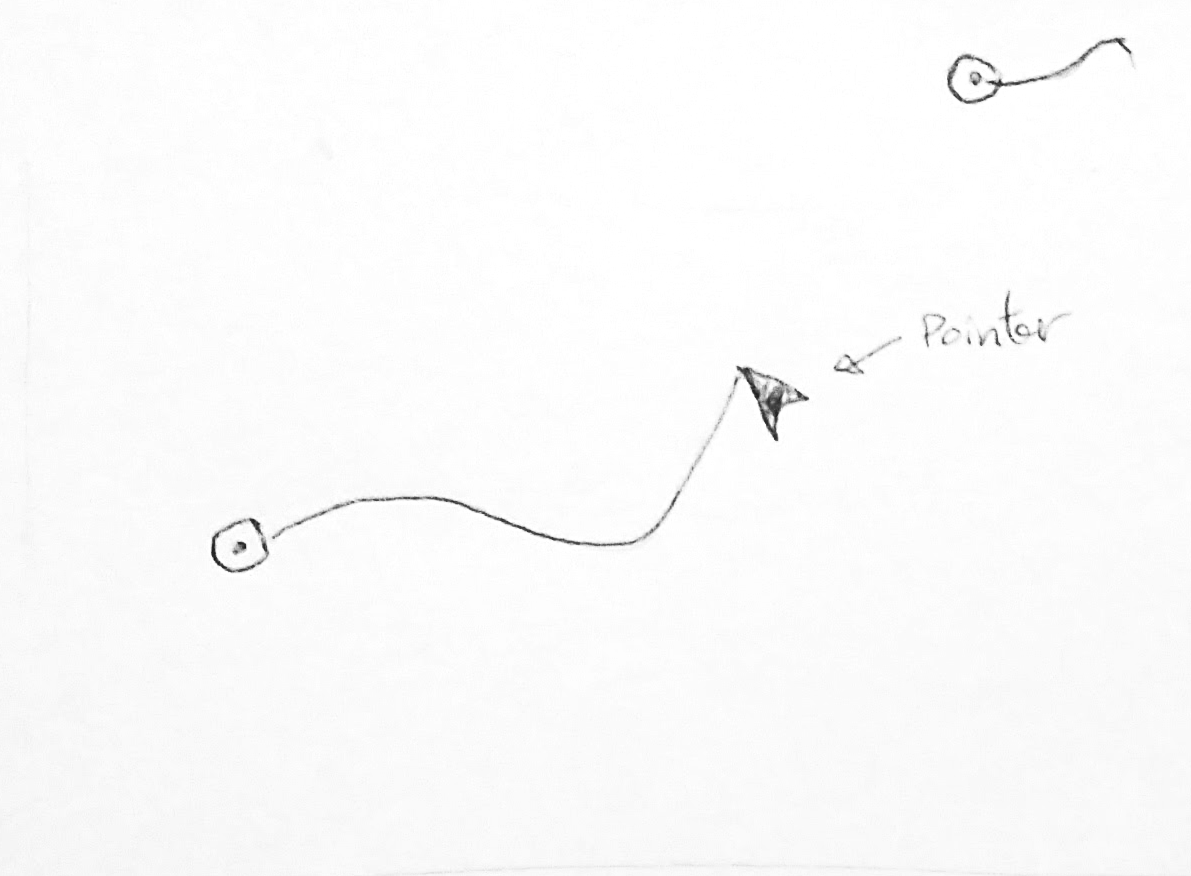
\includegraphics[width=\textwidth]{./charts/images/attractor-01.png}
        \caption{User starts note by dragging left to right}
    \end{subfigure}
    \hfill
    \begin{subfigure}{0.475\textwidth}
        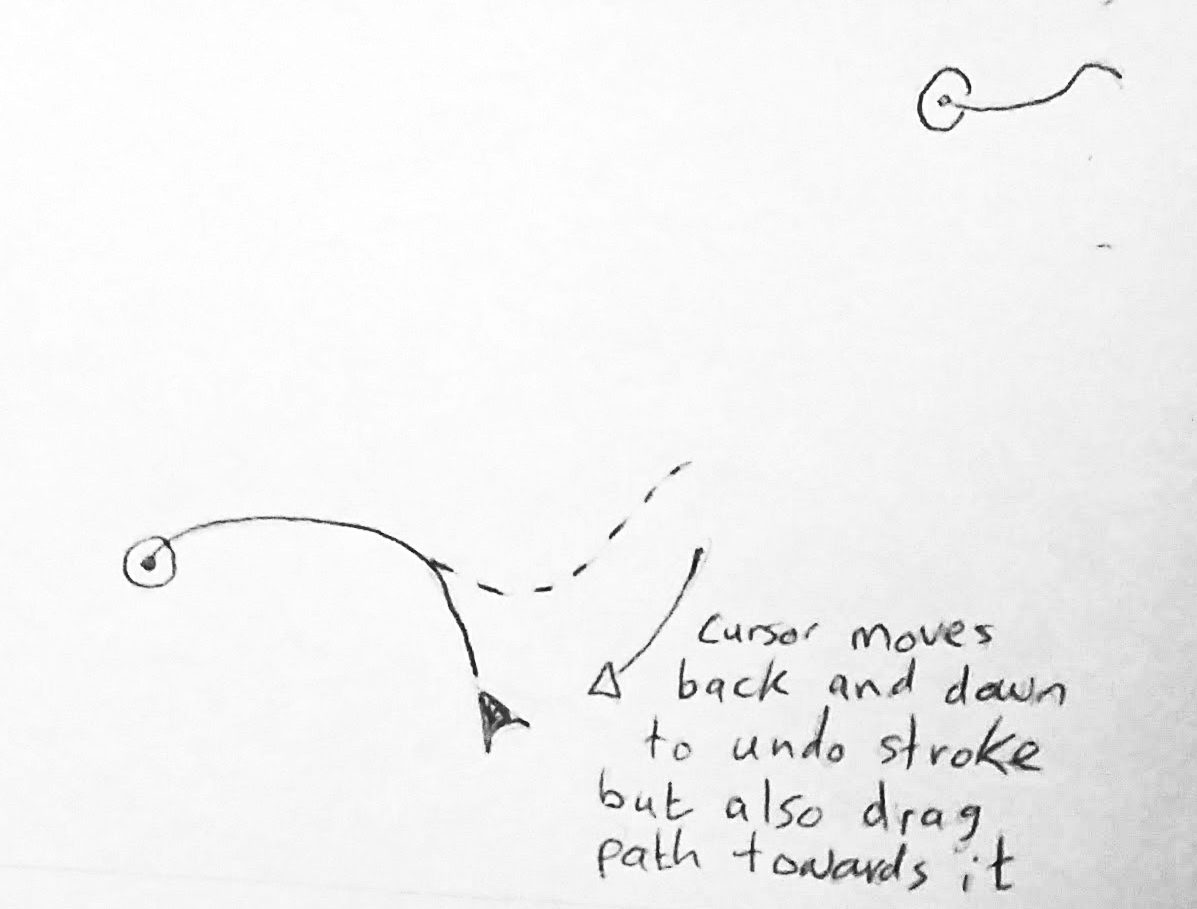
\includegraphics[width=\textwidth]{./charts/images/attractor-02.png}
        \centering
        \caption{Dragging back clears note}
    \end{subfigure}

    \caption{Adding notes in SonicSketch}
    \label{fig:adding-notes-sketch}
\end{figure}
\label{org12d88e5}
\end{LATEX}


The sketch tool is the default tool that is activated when the user opens the
application. It enables the user to add notes by drawing them onto the screen.
The event is captured in the main canvas view and is initiated when the
user left clicks the mouse to trigger the following function:

\begin{footnotesize}
\begin{verbatim}
(defn pointer-down [{:keys [temp-obj active-preset]} evt]
  (let [pointer-point (.. evt -point)
        ;; Group circle and path are temporary shapes
        group         (js/paper.Group. (clj->js {:position 
                        [(.. pointer-point -x) (.. pointer-point -y)]
                                                 :pivot [0 0]}))
        circle        (js/paper.Shape.Circle. (clj->js {:fillColor "#ffffff"
                                                        :radius    5}))
        path          (js/paper.Path. (clj->js {:strokeColor   "#ffffff"
                                                :strokeWidth   2
                                                :fullySelected true
                                                :segments      [[0 0]]}))]
    (.. group (addChildren #js [circle path]))
    (reset! temp-obj {:path   path
                      :circle circle
                      :group  group
                      :loc pointer-point})))
\end{verbatim}
\end{footnotesize}

This function receives a hashmap with a reference to a ClojureScript atom to
store the temporary visualisation of the newly created note. This function uses
javascript interop to directly instanciate paper.js objects and add them to a
shared group.

As the user continues to move the cursor further points are added to the path
created in the \texttt{pointer-down} function. Some constraints however are placed on
the creation of the path and only points that are past the last previous from
left to right are added. If the users backtracks it lead to a deletion of
points, providing an on-the-fly undo like behaviour. 
\begin{footnotesize}
\begin{verbatim}
(defn pointer-move [{:keys [temp-obj active-preset]} evt]
  (when-let [{:keys [path group] :as temp-obj} @temp-obj]
    (let [pointer-point (.. evt -point)
          rel-pos       (.. group (globalToLocal pointer-point))]
      ;; Only add positive points relative to first
      ;; Remove points greater than pointer-points
      (when-let [last-seg (.. path getLastSegment)]
        (let [first-seg   (.. path getFirstSegment)
              first-point (-> first-seg .-point)
              last-point  (-> last-seg .-point)
              pointer-x   (.-x rel-pos)
              amp-env     (-> active-preset :envelope)
              stage-width (.. evt -tool -view -viewSize -width)
              max-width   (if (= (-> amp-env :sustain) 0)
                            (let [time (+ (-> amp-env :attack)
                                          (-> amp-env :decay)
                                          (-> amp-env :release))]
                              (-> time
                                  ;; Seconds to beats
                                  (* (/ js/Tone.Transport.bpm.value 60))
                                  (time->euclidian stage-width)))
                            nil)]
          (when (or
                 (nil? max-width)
                 (< pointer-x (+ (.-x first-point) max-width)))
            (-> path (.add rel-pos))
            (let [greater-segs (filter
                                #(> (-> % .-point .-x) pointer-x)
                                (.-segments path))]
                ;; Remove greater points
              (doseq [seg greater-segs]
                  (.removeSegment path (.-index seg))))))))))
\end{verbatim}
\end{footnotesize}

Completion of a note occurs when the user releases the button and to trigger the
\texttt{pointer-up} function:
\begin{footnotesize}
\begin{verbatim}
(defn pointer-up [{:keys [temp-obj active-preset stage-size]} evt]
  (let [{:keys [path circle group loc] :as temp-obj} @temp-obj]
    (.simplify path 10)
    ;; Send the actual note
    (dispatch [:note-add (-> (path->note path loc stage-size)
                             (assoc ,,, :preset active-preset)
                             ;; Use the color from the active preset
                             (assoc ,,, :color (:color active-preset)))] )
    ;; Remove temporary objects
    (.remove path)
    (.remove group)
    (.remove circle))
  ;; Unset temp obj
  (reset! temp-obj nil))
\end{verbatim}
\end{footnotesize}
This function simplifies the path by calling the paper.js \texttt{simplify} method on
the path object and dramatically reduces the amount of data captured while
preserving the basic characteristic of the user's stroke. Most importantly it
calls the re-frame \texttt{dispatch} function to add the note to the \texttt{app-db}. A
\texttt{path->note} function is used to convert the stroke from the domain of euclidean
space in the visual space of the canvas to the domain of time-pitch space for
use with the audio synthesis system. The \texttt{path->note} function can be seen below:
\begin{footnotesize}
\begin{verbatim}
(defn path->note [path first-point stage-size]
  "Main entry point to this namespace"
  (let [path-width (.. path -bounds -width)
        width      (:width stage-size)
        height     (:height stage-size)]
    {:freq        (domain/euclidean->freq (.. first-point -y) height)
     :onset       (domain/euclidean->time (.. first-point -x) width)
     :duration    (domain/euclidean->time path-width width)
     :velocity    0.5
     :enabled     true
     :probability 1.0
     :color       @(col/as-css (get colors (rand-int 100)))
     :height      (.. path -bounds -height)
     :width       (.. path -bounds -width)
     :envelopes   {:frequency {:raw     (paper-path->vec path [width height])
                               :sampled (paper-path->sample path stage-size)}
                   :vibrato   (reduce (fn [a b]
                                        (assoc a b [b 0]))
                                      (sorted-map) (range 11))}}))
\end{verbatim}
\end{footnotesize}
The domain of time-pitch is used to store the notes in memory and makes it
possible to maintain a relative relationship between the screen size and the
drawn notes.

The dispatched note event is handled by a re-frame \texttt{reg-event-db} handler which
describes the alteration that is required to be made to the \texttt{app-db}. It also
uses a series of interceptors, to perform validation of the \texttt{app-db} and to
remove some of repeated code from the event handler functions. Interceptors are
similar conceptually to middleware and is the place where all of the
side-effects arising from an event are actioned. Moving application side-effects
here ensures that they are isolated and the majority of the program can be kept
as pure functions. As can be seen the handler function is very simple:
\begin{footnotesize}
\begin{verbatim}
(reg-event-db
 :note-add
 note-interceptors
 (fn [notes [note-info]]
   (let [id    (allocate-next-id notes)
         note  (assoc note-info :id id)]
     (if (>= (:duration note) 0.001)
       (assoc notes id note)
       notes))))
\end{verbatim}
\end{footnotesize}
This does a simple check to make sure that note has a minimum duration and if so
alters the notes vector to include the new vector which will instruct re-frame
to update the \texttt{app-db} with this new state.

The structure of the note hashmap is defined using \emph{clojure.spec}, a core
Clojure/Clojurescript library to perform data validation. The note specs are
defined as follows:
\begin{footnotesize}
\begin{verbatim}
(s/def ::id int?)
(s/def ::freq float?)
(s/def ::onset float?)
(s/def ::duration float?)
(s/def ::velocity float?)
(s/def ::color string?)
(s/def ::note (s/keys :req-un [::id ::freq ::onset ::duration]
                      :opt-un [::velocity]))
\end{verbatim}
\end{footnotesize}

Although not specified here, notes also have an \texttt{envelopes} key that stores
frequency and vibrato envelopes:
\begin{footnotesize}
\begin{verbatim}
{:frequency {:raw [{:point [-0.01 99.7]
                    :handle-in [0 100]
                    :handle-out [0 99.8]}  ...
                   {:point [2.8 98.02]
                    :handle-in [-0.10 100.4]
                    :handle-out [0 100]}]
             :sampled [-0.36991368680641185
                       ;; ...
                       -2.172026174596564]}
 :vibrato {0 [0 0], ... 10 [10 0]}}
\end{verbatim}
\end{footnotesize}
The update in state puts re-frame's subscription system into action and any
views that are subscribed to the changed application state are now re-rendered.
The \texttt{graphics-notes} view for instance is subscribed to \texttt{:notes},
\texttt{:graphics-stage-width}, \texttt{:graphics-stage-height} and \texttt{:mode}:
\begin{footnotesize}
\begin{verbatim}
(defn graphics-notes []
  (let [notes         (subscribe [:notes])
        width         (subscribe [:graphics-stage-width])
        height        (subscribe [:graphics-stage-height])
        ....]
    (into [:Group]
          (map (fn [note]
                 ^{:key (:id note)} [graphics-note* ...]) @notes))))
\end{verbatim}
\end{footnotesize}
When a note is added this render function will run which will call the
\texttt{[graphics-note]} component for each of the notes, and update the visual
display of the screen to show the new note. A similar process happens in the
audio system except, in this case, new web audio nodes are created, timeline
events are queued up at the correct time and audio envelopes are setup that
trace the curve of the drawn lines.     
\begin{footnotesize}
\begin{verbatim}
(defn fm-synth [{:keys [out] :as props} & children]
  "FM synth"
  ;; The new synth is instanciated using js interop
  (let [synth (js/Tone.FMSynth. (clj->js (dissoc props :out)))]
    (reagent/create-class
     {:component-did-mount
      (fn []
        ;; The synth is connected to it's output (which is passed
        ;; in as a property to the component)
        (.. synth (connect out)))
      :reagent-render
      (fn [props & children]
        ;; The render function renders a dummy span dom element and
        ;; renders it's children and passing it's synth as the out
        ;; for these components.
        (into [:span]
              (map (fn [child]
                     (assoc-in child [1 :out] synth))
                   children)))
      :component-will-unmount
      (fn []
        ;; Here we dispose of the synth
        ;; This will happen when the parent note is removed or when
        ;; a live code reload happens
        (.. synth dispose))})))
\end{verbatim}
\end{footnotesize}
The above shows the \texttt{fm-synth} which sits at the heart of the audio generating
part of the system. Potential parent components of this would be audio effects
or the master bus. It's child components are comprised of note events and
envelopes that drive frequency changes over the course of note playback. The
composition of events, envelopes, synths, effects and channels is shown in
truncated form:
\begin{footnotesize}
\begin{verbatim}
;; Parent component is the project and
;; has settings such as tempo
[project {:project :settings}
 [master-bus {}
  ;; Master volume is set here
  [volume {:volume :settings}
   ;; Adds a simple reverb effect
   [reverb-effect {}
    [
     ;; First note
     ;; Each note has a vibrato effect
     [vibrato-effect {}
      ;; Envelope to control vibrato depth
      [timeline-evt evt
       [envelope {:param "depth"
                  :env   vib-env}]]
      ;; The fm synth that generates the signal
      [fm-synth (get-in evt [:preset])
       ;; Timeline event that takes care of queuing
       ;; it's child components
       [timeline-evt evt
        ;; In this case a note
        [note {:note :settings}]
        ;; And a frequency envelope
        [envelope {:param "frequency"
                   :state state
                   :env   freq-env}]]]]
     ;; Second note
     [vibrato-effect {}
      ;; ...
      ]
     ;; ...
     ]]]]]
\end{verbatim}
\end{footnotesize}

\section{Editing notes}
\label{sec:org4b16edc}
\begin{footnotesize}
\begin{LATEX}
\begin{figure}[h]
\centering

\includegraphics[width=0.1\textwidth]{./assets/tools-panel.png}
\caption{SonicSketch tools panel}
\label{fig:sonicsketch-tools-panel}
\end{figure}
\label{orgee2873b}
\end{LATEX}
\end{footnotesize}

Once created, a number of editing operations can be performed on notes. Apart
from the \textbf{delete} action all of these operations involve first selecting the
note on the \textbf{mouse down} event, carrying out the editing of the note and
completing the action with the \textbf{mouse up} event. The particular tool can be
activated by clicking the icon the right-hand side of the screen (see figure
\ref{fig:sonicsketch-tools-panel}). Clicking one of these dispatches the
\texttt{:change-mode} event and changes the \texttt{app-db} to the specified mode as well as
setting the application to state \texttt{:pending}. Flowing from this change are a
number of changes:
\begin{enumerate}
\item The relevant paper.js tool is activated which will route further mouse
events to the appropriate dispatch handlers. For instance, when the
\texttt{:resize} mode is selected, \textbf{mouse move} events will be handled by
\texttt{:resize-tool-pointer-move}.
\item It updates the visual look of the cursor to remind the user which of mode
they are in.
\item A visual indicator is shown around the icon of the selected mode
\end{enumerate}
The overall effect of this is an activation of a number of different modes, each
of which will now be discussed.

In the case of deleting notes, the event is simply raised in the \textbf{click} event
of the note, which takes care of dispatching the \texttt{:note-delete} event. This is
handled by a very simple handler, \texttt{(dissoc notes note-id)} that instructs
re-frame to remove the note in question from the \texttt{app-db}. Similar to the
process that occurs when a note is added, the visual display is now updated to
no longer show the note. In addition, the signal generator, effects, envelopes
and events associated with the note are removed from the audio component tree.
React's lifecycle events take care of cleaning up any synths and
effects by calling their \texttt{dispose} methods.

Moving notes and resizing notes work very similarly and both follow the most
basic pattern described above of selection, manipulation, and completion. The
note selection event is raised from the note's \textbf{mouse down} event handler,
dispatching the \texttt{:note-select} event with the \textbf{note-id}. This updates the
\texttt{app-db} to set the \texttt{:active-note-id} to the received id, sets the app state to
\texttt{:active}, sets the note state to be \texttt{:active} and resets previously active
notes to state, \texttt{:normal}. This state update changes the visual display of the
active note to be highlighted by slightly lightening the colour of the note's
surrounding glow. More importantly, the note now becomes the active item on
which further user interactions are performed on. In the case of the \textbf{move} tool
the stored onset and pitch properties of the note are altered to reflect the
position of the user's mouse. This, in turn, updates the visual display of the
note and causes the audio system to re-queue the note events to the new onset
and pitch values. The \textbf{resize} tool, on the other hand, changes the size of the
starting node of the note and alters the velocity accordingly. The altered size
is calculated from the coordinates of the \textbf{mouse down} event and is clamped to a
maximum size that corresponds to the maximum velocity of the note.

The slightly more esoteric \textbf{probability} tool works in a very similar fashion to
the \textbf{resize} tools and again creates adjustments that work relative to the
initial \textbf{mouse down} coordinates. The visual effect that this creates, however,
is a dulling of the saturation of the note. Its effect is to add an element of
randomness and depending on how saturated the note is, it will cause the note to
randomly skip. The code for this is below:
\begin{footnotesize}
\begin{verbatim}
(let [enabled (-> (Math.random)
                  (<= ,, probability))]
  ;; Only trigger the note if enabled is true.
  ;; If probability is 1.0 will always be true.
  (if enabled
    (do
      (rf/dispatch [:note-enable id])
      (some-> out
              (.triggerAttackRelease ,,, freq (prep-time dur) t velocity)))
    (rf/dispatch [:note-disable id])))
\end{verbatim}
\end{footnotesize}
If the probability is fully saturated (corresponding to \texttt{1.0}, the default
value), the note will play on every loop. If, however, it is below this it will
skip in a random but probabilistic fashion, adding a small amount of
stochasticism to playback.

The vibrato tool is the most complex in its implementation and involves a small
popup UI element that allows the user to draw in a vibrato envelope which is
visually reflected in the note lines as an overlaid sinewave. After selection
occurs, in the usual way, \textbf{mouse move} events dispatch to the
\texttt{:vibrato-continue} handler which updates a vibrato modulation parameter in the
note, a single float value that represents the current real-time vibrato value.
This modulation parameter is passed back to the view through properties which
triggers a \texttt{:component-did-update} function call. It is here that a dispatch is
made to the \texttt{:vibrato-envelope-point} to create the envelope point. The reason
for the back and forth between the view and the event handlers is to allow the
event handlers to manage the state changes but deal with the specifics of the
geometry of the vibrato overlay in the view. 

A visual overlay is shown to the user when a vibrato action is started, that
shows a 10 point envelope, whose points are all set to \texttt{0.0} by default. The
user can then drag varying heights at various points on the horizontal axis
and create the time-varying vibrato envelope. This envelope is visualised (and
remains visible after the vibrato operation has completed) with a sinewave that
tracks the curve of the frequency envelope and varies its amplitude depending on
the strength of the vibrato at that particular point. The code to achieve this
is below:
\begin{footnotesize}
\begin{verbatim}
(->> (range 0.0 1.0 0.01)
     (map #(vector % (get-pos-of-curve-at-time curve %)))
     (map  (fn [[time p]]
             (let [norm          (.. curve (getNormalAt time))
                   loc           (.. curve (getLocationAtTime time))
                   relative-left (- (.. loc -point -x) left)
                   idx           (->
                                   ;; Normalize
                                   (/ relative-left width)
                                   ;; Mult by amp-env count
                                   (* (count amp-env))
                                   ;; Add amp-env starting point
                                   (+ (-> amp-env (first) (first)))
                                   ;; Round it off
                                   (Math/round))
                   amp           (-> (get amp-env idx)
                                     (second))]
               ;; Amp is here
               (sine-eq-along-vec time p norm (* amp 100) l)))))
\end{verbatim}
\end{footnotesize}

\chapter{Secondary functionality}
\label{sec:org3192fc0}
Aside from the core functionality of note creation and editing, a number of
other use cases were covered in the implementation. This includes transport
controls, to allow the user to start and stop playback; some simple animation to
show which notes are being played and to tighten the link between the visuals
and the audio; undo and redo functionality; a fullscreen toggle; save and load
functionality. Some of these extra features were made more straightforward than
would normally be the case due to the architecture of placing the state in a
single place, the re-frame \textbf{app db}.

Both the transport and the fullscreen mechanism consisted of a simple FSM whose
transitions are caused by user actions. The transport state machine responds to
both the \textbf{play toggle} button click and \textbf{spacebar} keypresses to toggle its state
between playing and stopped and based on this, triggering playback in tone.js.
The fullscreen FSM transitions occur not only when the user clicks the
fullscreen button but also when the browser fullscreen status changes. This
keeps the UI in a correct and consistent state at all times, regardless of how
the state is reached.

Undo/redo and save/load functionality was relatively straightforward to
implement for the reasons mentioned above (centrally located state) as well as
the ease of serialising ClojureScript data. Adding undo/redo was as easy as
adding an additional dependency and adding it as an interceptor to any events
that needed to be undoable such as adding or deleting notes. The particular
parts of the app state that needed to be restored were also configured and only
included the \texttt{notes} collection and the \texttt{tempo}. The same two elements were
saved and restored by the save/restore functionality which worked by serialising
this data as a string and restoring with a single function call to
\emph{ClojureScript}'s \texttt{reader/read-string}.

Some simple animation was added to playback to increase heighten the connection
between visuals and audio. To achieve this, the \texttt{:note} subscription is itself
subscribed to \texttt{:playback-beat} a reactive value that is kept up to date via the
use of events that fire on every animation frame. The subscription checks if the
playback head is within the notes range and if so sets its \texttt{:playing} property
to \texttt{true} and updates \texttt{:playback-time} to reflect the position of the playback
head in the note. Similar to any other changes in state, the note views react to
this and updates visual content accordingly to create the animation.
\begin{footnotesize}
\begin{verbatim}
(rf/reg-sub
 :note
 :<- [:notes-raw]
 :<- [:playback-beat]
 (fn [[notes playback-time] [_ id]]
   (let [{:keys [onset duration] :as note} (get notes id)
         end-time                          (+ onset duration)]
     (let [updated-note (if (and
                             (> playback-time onset)
                             (< playback-time end-time))
                          (-> note
                              (assoc ,,, :playing true)
                              (assoc ,,, :playback-time (- playback-time onset)))
                          (if (true? (-> note :playing))
                            (assoc note :playing false)
                            note))]
       updated-note))))
\end{verbatim}
\end{footnotesize}

\chapter{Conclusion}
\label{sec:org2d6b8d0}
This chapter outlined the development process that took place to bring
SonicSketch to life. The early prototype work was detailed, in addition to the
web port of SonicPainter, all work that contributed conceptually to the final
artifact. The setup of the technical architecture that brings together tone.js,
React, ClojureScript, Reagent and Paper.js was outlined. An in depth description
of the primary functionality that enables users to draw and edit notes on the
screen was given, followed by a more brief look at secondary functionality such
as undo, saving and note animation.


\newpage
\part{Evaluation}
\label{sec:org3d36c3f}
\chapter{Introduction}
\label{sec:org700267d}
An evaluation of the application will now be given. This is based on
self-assessment, user feedback and a usability questionnaire that polled a small
number of participants. User feedback was garnered at an exhibition that
showcased the application. More informal ongoing feedback also identified some
issues that were fixed in the final version of the application, in addition to
some that weren't.

\chapter{Assessment}
\label{sec:orgdcc7331}
\section{System architecture}
\label{sec:orgfd45488}
Overall, the chosen set of technologies worked very well and supported the
technical requirements of the project. The use of recently released and beta
versions of software libraries involved a good deal of time investment. Once
this was setup, however, the live coding workflow enabled easy experimentation
and proved invaluable when implementing complex features such as the vibrato
overlay. The transparent data oriented approach of ClojureScript aided in
debugging and made it straightforward to add advanced features such as undo/redo
and save/load.

\section{Core functionality - sketching notes}
\label{sec:org61160a8}
Adding notes was quite an easy concept for users to grasp and were observed to
quickly start making marks on the screen. Some users experienced confusion or
weren't aware of how to play these back initially. Once they managed to play the
audio back and understood the general nature of the sounds being created, a
common request was to clear the screen to start over. After this, they would
start experimenting with layering up different sounds on top of each other.
Oftentimes abstract visual patterns emerged and it seemed the visual feedback
played as much, if not more, of a role than the audio, in what was drawn on the
screen. Perhaps some real-time audio feedback might balance this out more. The
version that was tested required that notes are drawn from left to right,
causing some initial confusion for users. A future version will remedy this and
allow for both directions. The woodblock timbre only allows short lines to be
drawn as the sound isn't sustained and quickly decays after its initial attack.
This proved to be another source of confusion for users and indicates that it
may be inconsistent with other parts of the UI.

\section{Timbre selection}
\label{sec:orge47c59c}
Timbre selection is provided by clicking on one of the four coloured symbols to
the left of the screen. The regular geometric shapes represent harmonic shapes
and the more chaotic shapes represent non-harmonic sounds. Users did not seem to
make this connection though. After sketching some notes and hearing the various
timbres, most users were able to make the connection and to develop an intuitive
relationship between the visual appearance and the audio result. Some users felt
that the integration of timbre selection was a little flawed. When a tool other
than the sketch tool was in use, and a timbre selection was made, the
expectation was that it would return to the sketch tool. Instead, it stayed on
the same tool but just changed the timbre. This was updated in the final version
to reflect this expected behaviour. Another suggestion was to use icons that
represent the instrument rather than the more abstract icons present in the UI.
It was decided though that this would lead to an expectation of more realistic
sounds and, thus, was avoided, however.

\section{Vibrato}
\label{sec:org2166e0d}
Similar to tools other than the default sketch tool, the vibrato tool was not
heavily used by users and it was rarely discovered without some instruction.
Once discovered though, most users were able to operate it after one or two
attempts. The overlaid envelope graphic, while visually appealing in itself,
doesn't fit the sketching metaphor very well and doesn't depart very far from
what would be found in a traditional DAW. The resulting visualisation on the
notes helps to tie it back in with the sketching theme. Ideally, the user should
not see an overlay and instead directly adjust the visualisations on the note.
Unfortunately, these visualisations weren't executed perfectly either and are
applied slightly unevenly along the path of the note. It is a definite
improvement on those present in SonicPainter though.

\section{Other tools}
\label{sec:orgcfb4409}
Of the other available tools, delete and move were the most used. An initial
usability issue was the accurate click required to target the particular note to
be adjusted. Adding a glow effect to the notes remedied this to some degree and
gave a slightly larger area to click on. Apart from this, there weren't any
notable usability issues with either the delete or the move tools. The resize
and probability tools were the least seldom used and when they were used, posed
some difficulties for the user. They both worked on the principle of clicking on
the note in question and then dragging in or out to alter the value. The drag
motion didn't factor in the current value but was, rather, an absolute value
defined by the point that the user clicked and the distance to the user's mouse
pointer. Depending on the previous value, this caused a visual jump. In the case
of the probability tool, the change in saturation is quite subtle and the
changing colours may be difficult for the user to notice. The resize tool, which
adjusted the velocity, only changed the node size and not the overall size of
the graphic. This made it slightly unintuitive and confusing for the user,
perhaps contributing its low usage.

\section{Performance issues}
\label{sec:org0bf4b0f}
The application requires a reasonably fast and modern computer to run in a
usable state. However, even with fast hardware, complex heavily populated
sketches lead to audio and animation glitches. Some optimisations were made to
improve this. The primary adjustment was to add a \texttt{should-component-update} to
the \texttt{graphic-note} component. This gets called by the React system to check if
the component should re-render and is normally not needed for Reagent apps as it
supplies a default version. However based on performance testing with Google
Chrome Developer tools it could be seen that a large amount of scripting was
occurring on every frame (see figure fig:performance). This was the particularly
the case when the note count went beyond a dozen or so. Introducing the custom
\texttt{should-component-update} method reduced these renderings to an absolute minimum
bringing a significant performance boost.

Even with this improvement performance is still an issue. This is largely due to
the architectural decision to instantiate a new instrument for each note.
Potential improvements to this could be to:
\begin{itemize}
\item Render content as audio at certain points by using an \texttt{AudioWebWorker}, a Web
Audio API tool that allows rendering audio concurrently to a buffer. This
would alleviate some of the burden on the CPU by decreasing the amount of
audio generation it has to do.
\item Use Web Assembly, a relatively recent Web technology that allows optimized C
and C++ code to be compiled and run efficiently in the browser
\cite{adenot_web_2017}. Current versions of both Csound and Faust (a
functional audio programming language) can be compiled to run in the browser.
The author was able to run a Csound version of John Chowning's ``Stria''
smoothly on a smartphone's web browser.
\item Use hardware accelerated graphics to further ease the burden of the CPU and
improve visual display and animation.
\end{itemize}

\chapter{User testing and feedback}
\label{sec:orgcdde6a8}
\section{Usability questionnaire}
\label{sec:orge61aeb6}
The System Usability Scale (SUS) is usability questionnaire that uses a Likert
scale to give an indication of the how easy the application is to use. It poses
a number of questions designed to provoke extreme responses either in favour of
or against the proposition. Some examples of these are:
\begin{itemize}
\item I think that I would like to use this system frequently
\item I found the system very cumbersome to use
\end{itemize}
The original introduction of the SUS questionnaire stated that the individual
questions are meaningless and the results must be taken as a whole to give a
unidimensional usability scoring \citep{brook_sus_1995}.
\citet{lewis_factor_2009} have shown that this can be broken into two
dimensions, however, usability and learnability. This helps to gauge how
beginner friendly the application in addition to how generally usable it is.

\begin{table}[htbp]
\caption{\label{tab:org3ede874}
Results of SUS questionnaire}
\centering
\begin{tabular}{lr}
Factor & result\\
\hline
Learnability & 92\\
Usability & 83\\
Overall system satisfaction & 85\\
\end{tabular}
\end{table}

The final score that the system got was 85 out of 100. Learnability scored
higher than general usability, getting a total of 92 while general usability
came in below that, with a score of 83. This gives a strong indication that the
concepts and presentation of the app are easily grasped by novice users and that
the general perceived usability is very high. Despite the fact that the number
is scored out of 100 (with 100 being the highest score) it should not be
interpreted as a percentage. \citet{sauro_measuringu:_2011} has developed a
grading system based on the results of over 500 tests, suggesting a grade of A
to F, with A being the highest (figure fig:sus-grades). A score of 68 is average
and would give a grade of C. Anything above 80.3 is an A grade and according to
\citet{sauro_measuringu:_2011}, the point that users are more like to start
sharing with family and friends. Therefore, by this metric, SonicSketch achieves
a Grade A for overall system satisfaction, usability and for learnability.

Some caveats apply, however. The application was tested on a small group of
participants (15), most of whom were quite familiar with working with audio and
music applications. They were also colleagues of the author which may have
caused a bias towards positive feedback. Nonetheless, the indication was that
the application was straightforward and easy to start using, and provides a good
basis for future work.

\section{General feedback}
\label{sec:orga3b7034}
\begin{LATEX}
\begin{figure}[h]
\centering
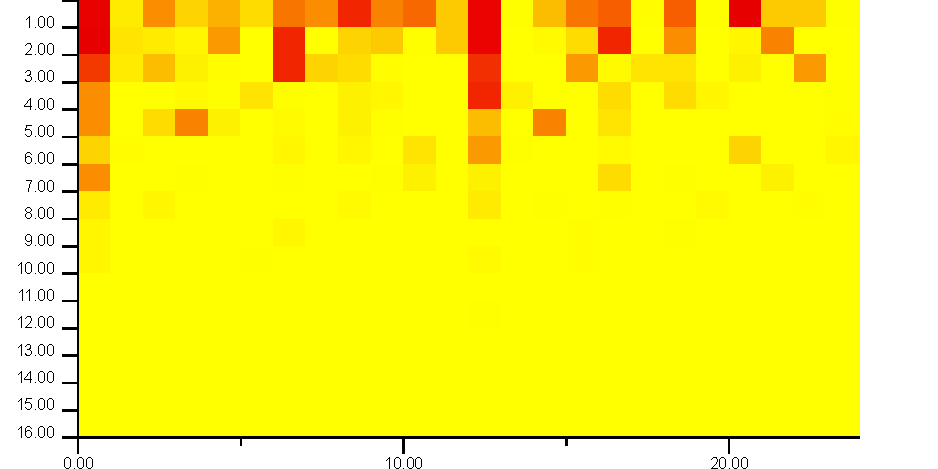
\includegraphics[width=1.0\textwidth]{./assets/hm-yellow-red.pdf}
\caption{Heat graph displaying note start points}
\label{fig:note-onset-hm}
\end{figure}
\label{org996ba97}
\end{LATEX}
\begin{LATEX}
\begin{figure}[h]
\centering
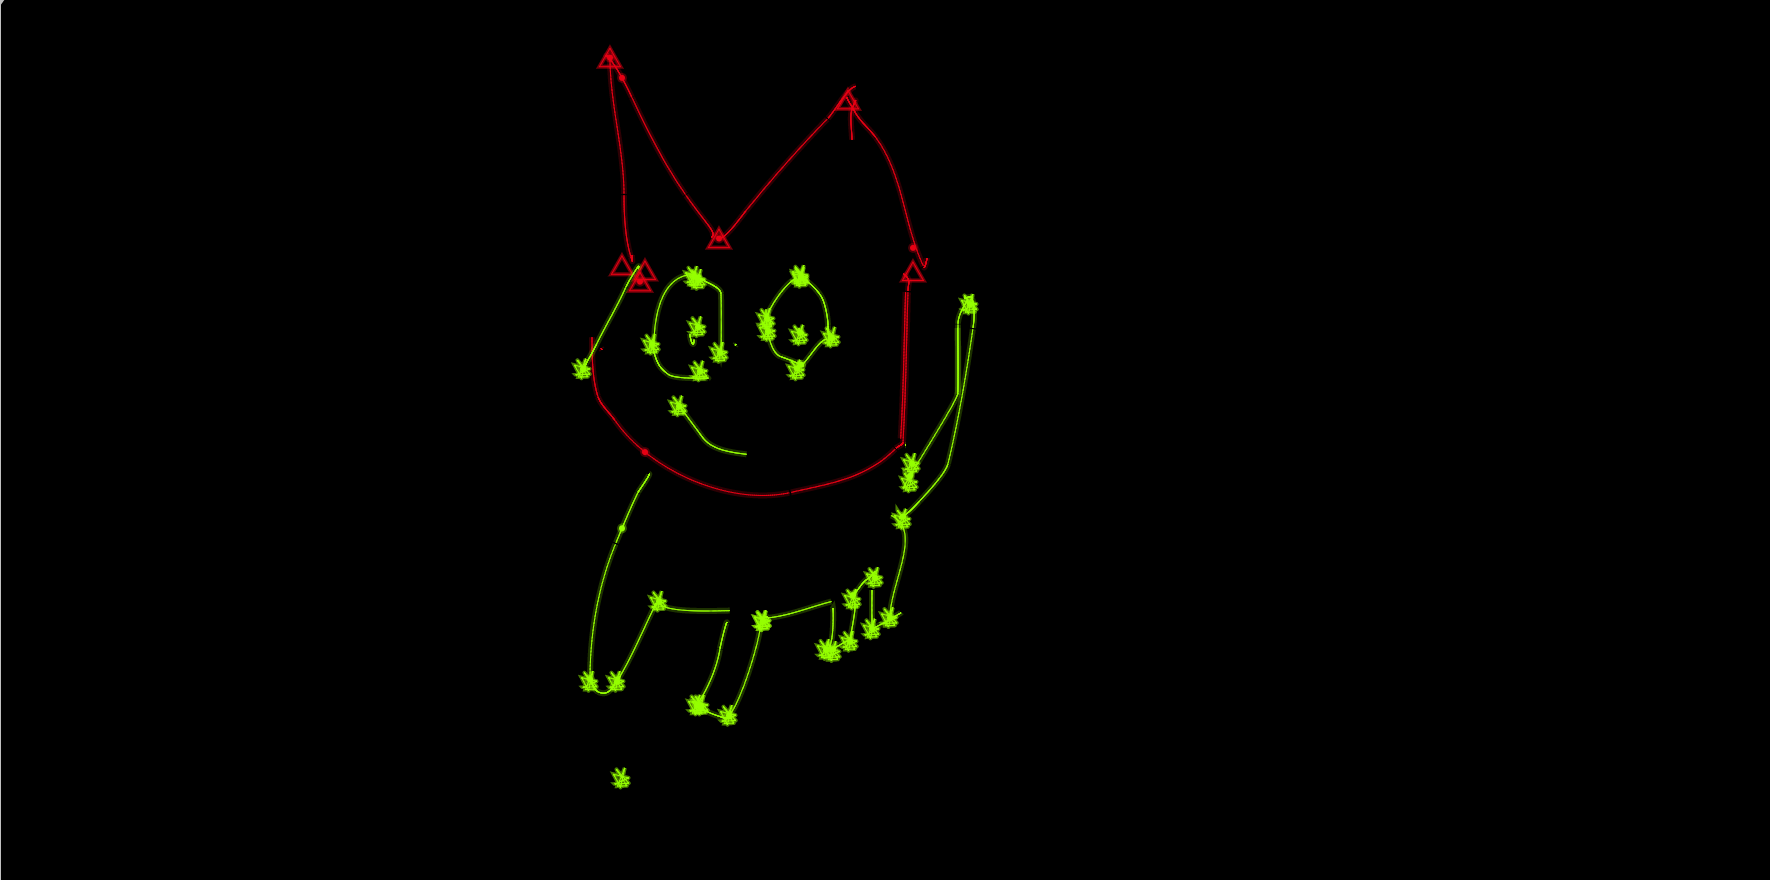
\includegraphics[width=1.0\textwidth]{./assets/exhibit-cat.png}
\caption{Some exhibit participants managed to draw figurative artwork!}
\label{fig:exhibit-cat}
\end{figure}
\label{orgb8b1014}
\end{LATEX}
Overall the feedback from both the questionnaire and at the exhibition was
positive with users reporting that it was a ``fun and enjoyable experience'' and
that they ``\ldots{} could play with [it] for ages.'' A number of testers suggested
that it would work well for sound design and cartoon sound effects in
particular: ``Really really fun! Can really see the benefit for sound design type
scenarios, animation films and the like.'' Another recurring comment was that it
would be interesting if you could sign your name and see what hear your sonic
signature. Unfortunately, the app isn't able to give interesting results in this
regard but it did show that users were engaging well with the concept of sonic
sketching. Another user commented: ``I enjoyed exploring how the different tools
affected the audio and I liked trying to layer more and more sounds on top of
one another.'' Again, this shows good engagement while at the same time pushing
the prototype software slightly beyond its limits as it struggled to play back
the ever increasing amount of audio material. A number of Sonic Sketches are
presented that showcase the diverse approaches taken, with some users achieving
figurative representations and another managing to (almost) sign her name
(fig:user-sonic-sketches).

\chapter{Conclusion}
\label{sec:org027da04}
This chapter presented a critical assessment of the final application that
factored in user testing and feedback. Each of the major features of the app
were assessed in terms of their success in contributing to the overall
application experience. As was discussed, some features worked well and didn't
incur any major friction in usage whereas others leave room for improvement.
Performance issues were discussed along with some potential remedies for these.
Finally, the SUS usability survey was discussed along with general feedback
received from users.

\newpage
\part{Conclusion and further work}
\label{sec:org794038c}
The dominant metaphors that underpin the modern DAW were discussed. Its
potential restrictiveness in some situations was illustrated with an example
composition. An alternative realisation was discussed using the Csound audio
programming language. The alternative metaphor of sketching was then explored
from a historic perspective to the more recent example of SonicPainter by
William Coleman. A more detailed critique of SonicPainter followed that
identified the key areas that SonicSketch would address. The core pieces of
technology being used in the application were then broken down along with
reasons for their choice. SonicSketch, an application that brings graphic
synthesis to the modern web browser, was then described both in its
functionality and underlying implementation. Finally, the resulting project was
evaluated both from a self-assessment and a user perspective.

\chapter{Future work}
\label{sec:orgedab749}
As such, there is an endless scope for improvements and features that could be
made and the following represents some of these:

\begin{description}
\item[{Performance improvements}] As is mentioned in the previous chapter, the
application requires some performance improvements to make it a viable
musician's tool. Ideally, the app should be able to run on mobile devices,
as the uncluttered interface would be a good match for the limited screen
size.
\item[{Larger structures}] The app doesn't offer any facility for larger structures.
It would be interesting to explore how the sketching metaphor could
translate to working at the arrangement level by perhaps introducing a
level of recursion and allowing the user to sketch sketches.
\item[{Micro structures}] The preset timbres are a serious limitation to the current
version. Taking inspiration from the UPIC, sonic flexibility could be
greatly increased by allowing users to define timbres by sketching
waveforms and envelopes.
\item[{Zooming and panning}] This would allow users to focus on particular parts of
their sonic sketches and navigate through the sketch similarly to graphic
editors like Photoshop.
\item[{More input devices}] Work was carried out to integrate graphics tablets into
the application using the W3C Pointer API, a relatively new API that
provides comprehensive support for multiple input devices including
multitouch and graphics tablets (with pressure support and angle data).
Unfortunately, it wasn't included in this version and is left for future
work.
\item[{Grids}] While the freeform gridless canvas of the current version is fun to
play with, an optional grid would allow for more precise control.
Rather than only offering the chromatic grid, only suited to western
music, however, a number of different grids could be made available.
Perhaps a psychoacoustic grid based on the Bark scale could provide
an interesting alternative or a grid based on Setharthes' dissonance
curves.
\end{description}

The presented application represents a very small step in exploring the metaphor
of sonic sketching. A virtually bottomless source of inspiration can be found in
the many systems that have gone before it, some of which exist, and some of
which can only be enjoyed through textual description, images and if, we're
lucky videos. The modern web browser represents a unique opportunity to
experiment with and develop these alternative approaches to music interface
design in an environment that offers unprecedented ease of access for its users.

\newpage

\part{Appendices}
\label{sec:org6f41a0f}
\chapter{Appendix A - SUS Questionnaire}
\label{sec:orgf66f036}
The following is the list of propositions that the tester must grade from
strongly agree to strongly disagree.
\begin{enumerate}
\item I think that I would like to use this system frequently
\item I found the system unnecessarily complex
\item I thought the system was easy to use
\item I think that I would need the support of a technical person to be able to use this system
\item I found the various functions in this system were well integrated
\item I thought there was too much inconsistency in this system
\item I would imagine that most people would learn to use this system very quickly
\item I found the system very cumbersome to use
\item I felt very confident using the system
\item I needed to learn a lot of things before I could get going with this system
\end{enumerate}

\newpage

\part{Bibliography}
\label{sec:org42f2ba0}
\end{document}